\documentclass[12pt]{article}
\usepackage[hmargin=1.4in,vmargin=1.4in]{geometry}
\bibliographystyle{ecta}
\usepackage[pdftex]{graphicx}
\usepackage[update,prepend,outdir=../output/figures/]{epstopdf}
\usepackage{subfigure}
\usepackage{amsthm}
\usepackage{amsmath}
\usepackage{amsfonts}
%\usepackage{mathbfol}
\usepackage{xcolor}
\usepackage{tcolorbox}
\usepackage{enumerate}
\usepackage[onehalfspacing]{setspace}
\usepackage{multirow}
\usepackage{cancel}
% \usepackage{epstopdf}
\usepackage{natbib}
\usepackage{bm}                                                                                                                                                                                                                    
%\usepackage{chngcntr}
\usepackage{apptools}
\usepackage[multiple]{footmisc}
\usepackage[hidelinks,hyperfootnotes=false]{hyperref}
\usepackage{fancyhdr}
\usepackage{footnote}

\usepackage{afterpage}
\usepackage{floatrow}
\usepackage{array}
\usepackage{xr}
\usepackage{adjustbox}
\usepackage{pdflscape}
\usepackage{array}
\externaldocument{\jobname_app}
\makesavenoteenv{tabular}
\makesavenoteenv{table}
\usepackage{datetime}
\bibliographystyle{ecta}
\allowdisplaybreaks

%\usepackage{mathtools}
%\linespread{1.2}

%\newtheorem{ass}{Assumption}
\newenvironment{ass}[2][Assumption]{\begin{trivlist}
\item[\hskip \labelsep {\bfseries #1}\hskip \labelsep {\bfseries #2}]}{\end{trivlist}}
\newtheorem{conj}{Conjecture}
\newtheorem{defn}{Definition}
\newtheorem{prop}{Proposition}
\newtheorem{cor}{Corollary}
\newtheorem{lem}{Lemma}
\newcommand{\tunderbrace}[1]{\underbrace{\textstyle#1}}
\newcommand{\toverbrace}[1]{\overbrace{\textstyle#1}}
\makeatletter
\newcommand{\vast}{\bBigg@{3}}
\newcommand{\Vast}{\bBigg@{4}}
\makeatother

\newcolumntype{L}[1]{>{\raggedright\arraybackslash}m{#1}}
%\newcolumntype{L}[1]{>{\raggedright\let\newline\\\arraybackslash\hspace{0pt}}m{#1}}
\newcolumntype{C}[1]{>{\centering\arraybackslash}m{#1}}
\def\sym#1{\ifmmode^{#1}\else\(^{#1}\)\fi}
\newdateformat{monthyeardate}{%
  \monthname[\THEMONTH] \THEYEAR}

\AtAppendix{\counterwithin{lem}{section} \counterwithin{defn}{section} \counterwithin{prop}{section} \counterwithin{cor}{section}}

\newcolumntype{R}[2]{%
    >{\adjustbox{angle=#1,lap=\width-(#2)}\bgroup}%
    l%
    <{\egroup}%
}
\newcommand*\rot{\multicolumn{1}{R{45}{1em}}}% no optional argument here, please!


\begin{document}
\section{Numerical solution: main text}

\begin{table}[H]
\centering
\bgroup
\def\arraystretch{1.25}
\begin{tabular}{clcl} \hline
& Description & Value & Notes \\ \hline
$\psi$ & IES & 0.75 & \\ 
$\sigma$ & trade elasticity & 1.5 & \cite{backusetal1994} \\ 
$\varsigma$ & home bias & 0.4 & \cite{eatonetal2016} \\ 
$\nu$ & Frisch elasticity & 0.75 & \cite{chettyetal2011} \\ 
$\alpha$ & 1 - labor share & 0.33 & \\ 
$\delta$ & depreciation rate & 0.025 & \\ 
$\epsilon$ & elast. of subs. across workers & 20 \\ 
$\chi^{W}$ & Rotemberg wage adj. costs & 400 & $\approx \mathbb{P}(\mbox{adjust}) = 5 \enspace \mbox{qtrs}$ \\ 
$\phi^\pi$ & Taylor coeff. on inflation & 1.5 & \cite{taylor1993}  \\ 
$\underline{\varphi}$ & disaster shock & -0.10 & \cite{nakamuraetal2013} \\ 
$p$ & disaster risk & 0.4\% & $E[p] = 0.5\%$ (\cite{barro2006}) \\ 
$\rho^p$ & dis. risk persistence & 0.75 & $\rho(p) = 0.7$ \\ 
$\sigma^p$ & dis. risk std. dev. & 0.55 & $\sigma(p)/E[p] = 1$ \\ 
$\omega^d$ & safety skewness & 0.002 & $skew(\omega) = 6.1$ \\
$\rho^{\omega}$ & safety persistence & 0.4 & $\rho(\omega) = 0.3$ \\ 
$\rho^{p\omega}$ & corr. safety, disaster & 0.5 & $\rho(p,\omega) = 0.4$ \\ \hline 
\hline 

\end{tabular}
\egroup
\renewcommand\thetable{1}
\caption{externally set parameters}
\label{tab:ext}
\end{table}




\begin{table}[H]
\centering
\bgroup
\def\arraystretch{1.25}
\begin{tabular}{clclcc} \hline
& Description & Value & Moment & Target & Model   \\ 
\hline 
$\zeta^*$         & rel. pop.            & 1.6 & $y^*/(sy)$                                           & 1.6     & 1.6     \\ 
$\sigma^z$        & std. dev. prod.      & 0.002 & $\sigma(\Delta \log c)$                              & 0.5\% & 0.5\% \\ 
$\sigma^{F}$      & std. dev. rel. prod. & 0.005 & $\sigma(\Delta\log y^*)$                             & 0.8\% & 0.8\% \\ 
$\rho^{F}$        & persist. rel. prod.  & 0.9 & $\rho(y^*/y,y_{-4}^*/y_{-4})$                        & 0.6     & 0.5     \\ 
$\chi^x$          & capital adj cost     & 3 & $\sigma(\Delta \log x)$                              & 1.6\% & 1.6\% \\ 
$\beta^*$         & disc. fac. Foreign   & 0.9892 & $4 \mathbb{E} r$                                     & 2.0\% & 2.0\% \\ 
$\beta$           & disc. fac. Home      & 0.9887 & $nfa/(4y)$                                           & -23\% & -23\% \\ 
$\sigma^{\omega}$ & std. dev. safety     & 0.91 & $\rho_{-1}\left(r^e,r^* + \Delta \log q - r\right)$  & 0.5 & 0.5 \\ 
$\gamma^*$        & RRA Foreign          & 24 & $4 \mathbb{E} \left[r^e - r \right]$                 & 5.1\% & 5.2\% \\ 
$\gamma$         & RRA Home             & 21 & $\beta((\Delta nfa)/y,r^e - r)$                      & 0.5 & 0.6 \\ 
$\bar{b}^g$      & safe debt/agg. cons. & 0.127 & $b_{H,s}^*/(4y)$                                     & 3.8\% & 3.8\% \\ 
$\bar{\nu}$       & $\ell$ disutility    & 0.73 & $\ell$                                               & 1     & 1.0     \\ 
$\bar{\nu}^*$     & $\ell^*$ disutility  & 0.71 & $\ell^*$                                             & 1     & 1.0     \\ 
$\bar{i}$     & Taylor intercept Home & 0.49\% & $\log P/P_{-1}$                                           & 0.0\% & 0.0\% \\ 
$\bar{i}^*$     & Taylor intercept Foreign & 0.47\% & $\log P^*/P^*_{-1}$                                        & 0.0\% & 0.0\% \\ 
\hline 

\end{tabular}
\egroup
\renewcommand\thetable{2}
\caption{targeted moments and calibrated parameters}
\floatfoot{Notes: second moments are reported over quarterly frequency.  Data moments are estimated over Q1 1995 -- Q4 2019.  Model moments are computed by (i) simulating model for 20,000 quarters and discarding first 10,000 quarters; (ii) drawing 100 starting points from remaining 10,000 quarters; (iii) simulating 100 samples beginning from these starting points, with no disaster realizations in sample; (iv) computing moments for each sample and averaging across samples.}
\label{tab:cal}
\end{table}


\vspace{40pt}

\begin{figure}[H]
\centering
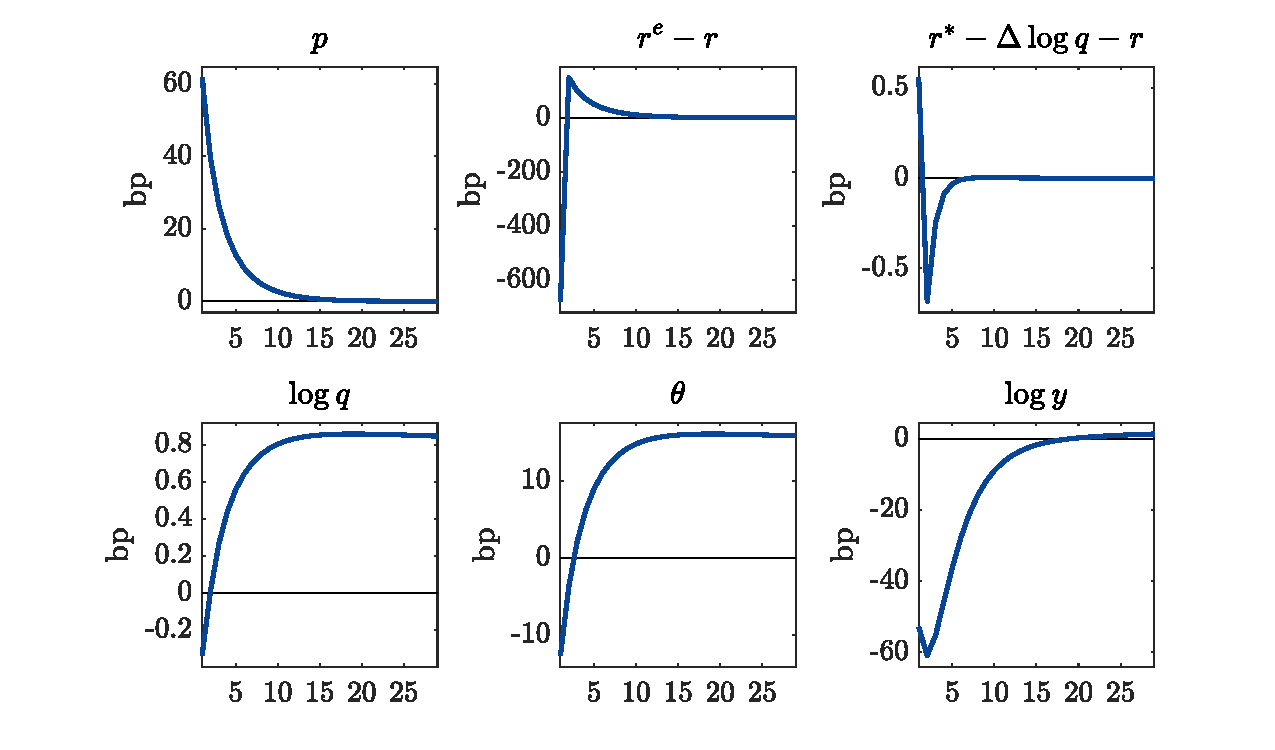
\includegraphics[width=\textwidth,clip=true,trim=0 0 0 0]{../output/figures/fig_2}
\renewcommand\thefigure{2}
\caption{effects of increase in disaster probability}
\floatfoot{Notes: impulse responses are average responses starting from 100 points drawn from ergodic distribution as described in note to Table \ref{tab:cal}.}
\end{figure}

\begin{figure}[H]
\centering
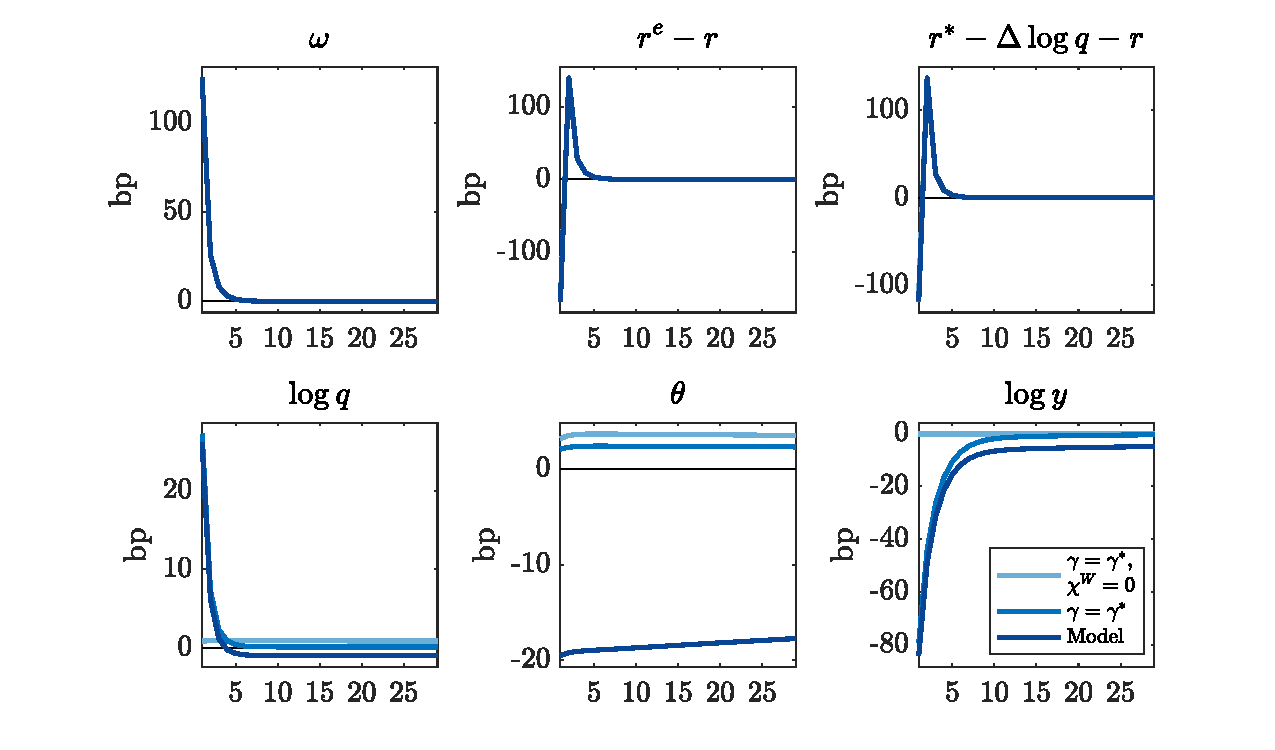
\includegraphics[width=\textwidth,clip=true,trim=0 0 0 0]{../output/figures/fig_3}
\renewcommand\thefigure{3}
\caption{effects of increase in safety}
\floatfoot{Notes: impulse responses are average responses starting from 100 points drawn from ergodic distribution as described in note to Table \ref{tab:cal}.}
\end{figure}

\begin{table}[H]
\centering
\bgroup
\def\arraystretch{1.25}
\begin{tabular}{l|cccc} \hline
  & Data & Model & No $\omega$ & $\gamma=\gamma^\ast$ \\ 
\hline 
$\beta(r_{t+1}^* - \Delta \log q_{t+1} - r_{t+1},\log y_t - \log y_{t-4})$ & $ -0.17$ & $ -0.11$ & $  0.00$ & $ -0.11$ \\ 
& (0.11) & & & \\ 
$\beta(r_{t+1}^* - \Delta \log q_{t+1} - r_{t+1},r_{t+1}^e)$ & $  0.23$ & $  0.06$ & $ -0.00$ & $  0.06$ \\ 
& (0.04) & & & \\ 
$\beta((\Delta nfa_{t+1})/y_t,r_{t+1}^* - \Delta \log q_{t+1} - r_{t+1})$ & $  1.38$ & $  1.45$ & $ -3.39$ & $  0.25$ \\ 
& (0.30) & & & \\ \hline 
\emph{Memo}: $(k-\kappa)/(4y)$ &  & $  59.8\%$ & $  50.2\%$ & $   0.1\%$ \\ 
\hspace{1.25cm} $b_H/(4y)$ & & $-102.5\%$ & $ 151.3\%$ & $  14.3\%$ \\ 
\hspace{1.25cm} $b_F/(4y)$ &  & $  19.8\%$ & $-224.6\%$ & $ -15.9\%$ \\ 
\hline 

\end{tabular}
\egroup
\renewcommand\thetable{3}
\caption{comovements in the international monetary system}
\floatfoot{Notes: data moments estimated over 1995 - 2019.  Standard errors are given in parenthesis.  First two rows use monthly data and thus \cite{hh1980} standard errors with 4 lags to correct for overlapping observations.  Model moments are computed as described in note to Table \ref{tab:cal}.}
\label{tab:comov}
\end{table}

\begin{table}[H]
\centering
\bgroup
\def\arraystretch{1.25}
\begin{tabular}{l|cccc} \hline
Moment & Data & Model & No $\omega$ & $\gamma=\gamma^\ast$ \\ 
\hline 
$\sigma(4r_t)$ & $   2.9\%$ & $   4.1\%$ & $   2.1\%$ & $   4.1\%$ \\ 
$\sigma(4[r_t^e - r_t])$ & $  33.6\%$ & $  17.2\%$ & $  11.2\%$ & $  17.5\%$ \\ 
$\sigma(4[r_t^\ast - \Delta\log q_t - r_t])$ & $  15.5\%$ & $   1.9\%$ & $   0.3\%$ & $   1.9\%$ \\ 
\hline 
$\sigma(\Delta\log q_t)$ & $   3.8\%$ & $   0.3\%$ & $   0.2\%$ & $   0.3\%$ \\ 
$\sigma(\Delta\log E_t)$ & $   3.8\%$ & $   0.4\%$ & $   0.2\%$ & $   0.4\%$ \\ 
\hline 
$\sigma(\Delta\log q_t, \Delta\log c^\ast_t - \Delta\log c_t)$ & $  0.10$     & $  0.91$     & $  0.92$     & $  0.97$     \\ 
\hline 

\end{tabular}
\egroup
\renewcommand\thetable{4}
\caption{additional second moments}
\floatfoot{Notes: data moments are estimated over Q1 1995 -- Q4 2019.  Standard errors are given in parenthesis.  Model moments are computed as described in note to Table \ref{tab:cal}.}
\label{tab:addmom}
\end{table}

\begin{table}[H]
\centering
\bgroup
\def\arraystretch{1.25}
\begin{tabular}{l|cccc} \hline
Moment & Data & Model & No $\omega$ & $\gamma=\gamma^\ast$ \\ 
\hline 
$\sigma(\Delta\log y_t)$ & $  0.59\%$ & $  0.61\%$ & $  0.44\%$ & $  0.60\%$ \\ 
$\sigma(\Delta\log y^\ast_t)$ & $  0.81\%$ & $  0.81\%$ & $  0.75\%$ & $  0.81\%$ \\ 
\hline 

\end{tabular}
\egroup
\renewcommand\thetable{5}
\caption{output volatility}
\floatfoot{Notes: data moments estimated over Q1 1995 - Q4 2019.  Model moments are computed as described in note to Table \ref{tab:cal}.}
\label{tab:yvol}
\end{table}

\begin{table}[H]
\centering
\bgroup
\def\arraystretch{1.25}
\begin{tabular}{l|cccc} \hline
Moment & Data & Model & No $\omega$ & $\gamma=\gamma^\ast$ \\ 
\hline 
$\sigma((\Delta nfa_t)/y_t)$ & $  11.0\%$ & $   3.3\%$ & $   1.6\%$ & $   0.8\%$ \\ 
$\sigma(nx_t/y_t)$ & $   1.0\%$ & $   1.0\%$ & $   0.8\%$ & $   0.8\%$ \\ 
$\sigma((\Delta nfa_t - nx_t)/y_t)$ & $  10.9\%$ & $   3.1\%$ & $   1.8\%$ & $   0.2\%$ \\ 
\hline 
$\Delta nfa/y$ & $  -2.8\%$ & $   0.2\%$ & $   0.1\%$ & $   0.0\%$ \\ 
$nx/y$ & $  -3.2\%$ & $  -0.6\%$ & $  -0.2\%$ & $   0.1\%$ \\ 
$(\Delta nfa - nx)/y$ & $   0.4\%$ & $   0.7\%$ & $   0.3\%$ & $  -0.1\%$ \\ 
\hline 

\end{tabular}
\egroup
\renewcommand\thetable{6}
\caption{U.S. net foreign asset volatility}
\floatfoot{Notes: volatilities in data estimated over Q1 2006 - Q4 2019 since BEA IIP data is available quarterly only after that date; means are estimated using annual data over Q1 1995 - Q4 2019.  Model moments are computed as described in note to Table \ref{tab:cal}.}
\label{tab:nfanxvol}
\end{table}

\begin{table}[H]
\centering
\bgroup
\def\arraystretch{1.25}
\begin{tabular}{l|ccc} \hline
  & Model  & No $\omega$ & $\gamma=\gamma^\ast$ \\ \hline 
\emph{As share of} $Var\left((\mathbb{E}_t - \mathbb{E}_{t-1})nfa_t\right)$: & & \\$Cov\left(-(\mathbb{E}_t - \mathbb{E}_{t-1})\sum_{h=1}^{500} \left(\prod_{i=1}^{h} \frac{1}{1+r_{t+i}^k}\right)nx_{t+h},(\mathbb{E}_t - \mathbb{E}_{t-1})nfa_t\right)$ & $  32.3\%$ & $  76.2\%$ & $  99.1\%$ \\ 
$Cov\left(-(\mathbb{E}_t - \mathbb{E}_{t-1})\sum_{h=1}^{500} \left(\prod_{i=1}^{h} \frac{1}{1+r_{t+i}^k}\right)val_{t+h},(\mathbb{E}_t - \mathbb{E}_{t-1})nfa_t\right)$ & $  67.6\%$ & $  23.8\%$ & $   0.9\%$ \\ 
$Cov\left((\mathbb{E}_t - \mathbb{E}_{t-1})\left(\prod_{i=1}^{500} \frac{1}{1+r_{t+i}^k}\right)nfa_{t+500},(\mathbb{E}_t - \mathbb{E}_{t-1})nfa_t\right)$ & $   0.1\%$ & $   0.1\%$ & $  -0.0\%$ \\ 
\hline 

\end{tabular}
\egroup
\renewcommand\thetable{7}
\caption{understanding U.S. external adjustment}
\floatfoot{Notes: moments are computed as described in note to Table \ref{tab:cal}, but including disaster realizations.}
\label{tab:extadj}
\end{table}

\begin{figure}[H]
\centering
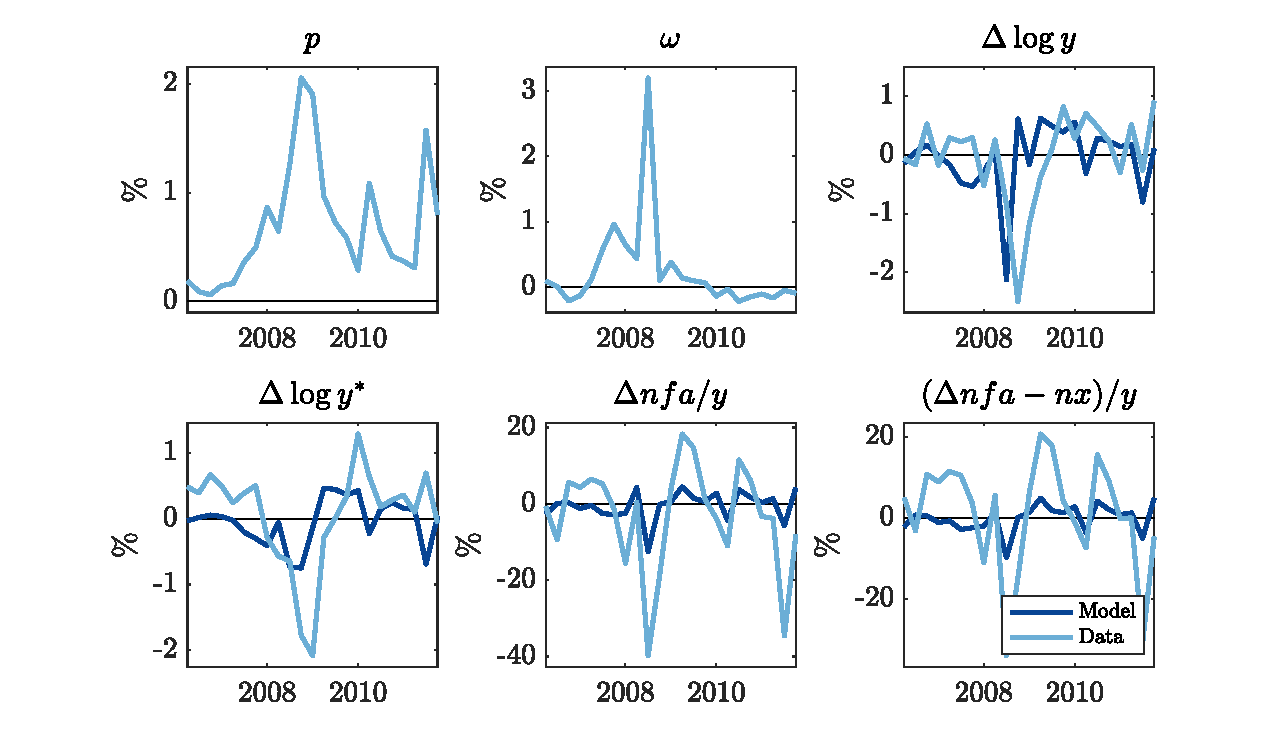
\includegraphics[width=\textwidth,clip=true,trim=0 0 0 0]{../output/figures/fig_4}
\renewcommand\thefigure{4}
\caption{simulation using observed $p$ and $\omega$ series}
\floatfoot{Notes: $p$ is from \cite{bl2021} and $\omega$ is from \cite{duetal2018} (demeaned).  Both are scaled to match volatilities of $p$ and $\omega$ in model.  Given these shocks, figure depicts average paths starting from 100 points drawn from ergodic distribution as described in note to Table \ref{tab:cal}.}
\label{fig:gr}
\end{figure}

\begin{table}[tb]
\centering
\bgroup
\def\arraystretch{1.25}
\begin{tabular}{l|C{21mm}C{18mm}C{19mm}} \hline
& & \multicolumn{2}{c}{Model} \\ 
& Data & Constant $i$ & Active Taylor \\ \hline
 \emph{Impact effects} & & &\\ 
 $\log E_t$ & $-72bp$ & $-100bp$ & $-18bp$ \\ 
 $\log P_t r_t^e$ &  $+151bp$& $+135bp$& $+29bp$ \\  
 $\Delta nfa_t/y_t$ & & $+436bp$& $+67bp$ \\ 
 $\Delta(nfa_t-nx_t)/y_t$ & & $+351bp$& $+63bp$ \\ \hline 
 \emph{Peak effects} & \\ 
 $\log y_t$ & & $+79bp$& $+11bp$\\ 
 $\log y_t^*$ & & $+21bp$& $+4bp$ \\ \hline 

\end{tabular}
\egroup
\renewcommand\thetable{8}
\caption{effects of dollar swap lines}
\floatfoot{Notes: data column are cumulative estimates from \cite{kl2023a} for March 19-20, 2020 announcements (Table 1 in that paper).  Model columns simulate a decrease in $\omega_t$ of $14bp$ starting from the average of the model's ergodic distribution.}
\label{tab:swapline}
\end{table}	

\section{Numerical solution: appendix}

\begin{figure}[H]
\centering
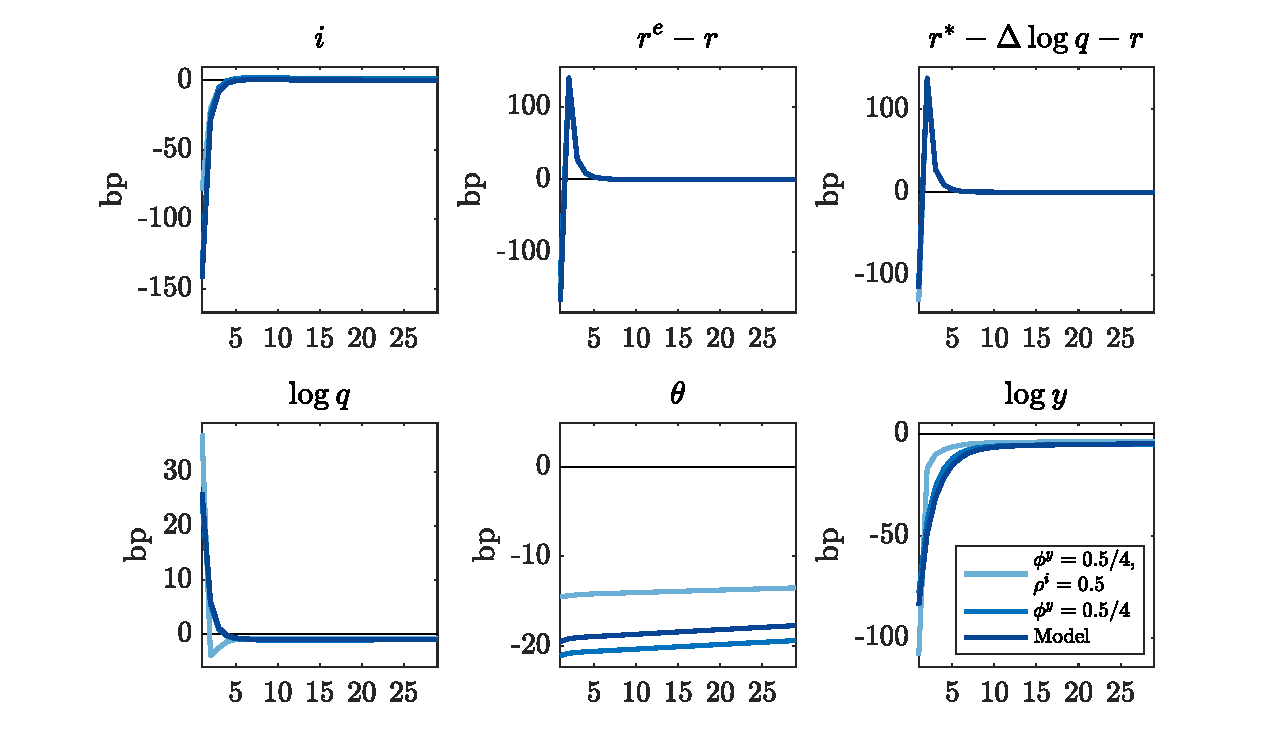
\includegraphics[width=\textwidth,clip=true,trim=0 0 0 0]{../output/figures/fig_5}
\renewcommand\thefigure{5}
\caption{effects of increase in safety under alternative monetary policy rules}
\floatfoot{Notes: impulse responses are average responses starting from 100 points drawn from ergodic distribution as described in note to Table \ref{tab:cal}.}
\end{figure}

\begin{table}[H]
\centering
\bgroup
\def\arraystretch{1.25}
\begin{tabular}{l|cccc} \hline
  & Model & $\phi^y=0.5/4$ & $\phi^y=0.5/4$, $\rho^i=0.5$\\ 
\hline 
$\beta(r_{t+1}^* - \Delta \log q_{t+1} - r_{t+1},\log y_t - \log y_{t-4})$ & $ -0.11$ & $ -0.10$ & $ -0.13$ \\ 
$\beta(r_{t+1}^* - \Delta \log q_{t+1} - r_{t+1},r_{t+1}^e)$ & $  0.06$ & $  0.06$ & $  0.08$ \\ 
$\beta((\Delta nfa_{t+1})/y_t,r_{t+1}^* - \Delta \log q_{t+1} - r_{t+1})$ & $  1.45$ & $  1.30$ & $  0.86$ \\ \hline 
\emph{Memo}: $(k-\kappa)/(4y)$ & $  59.8\%$ & $  51.9\%$ & $  37.7\%$ \\ 
\hspace{1.25cm} $b_H/(4y)$ & $-102.5\%$ & $-127.0\%$ & $ -72.5\%$ \\ 
\hspace{1.25cm} $b_F/(4y)$ & $  19.8\%$ & $  52.1\%$ & $  12.9\%$ \\ 
\hline 

\end{tabular}
\egroup
\renewcommand\thetable{9}
\caption{comovements under alternative monetary policy rules}
\floatfoot{Notes: moments are computed as described in note to Table \ref{tab:cal}.}
\label{tab:comov}
\end{table}

\begin{table}[H]
\centering
\bgroup
\def\arraystretch{1.25}
\hspace*{-2cm}\begin{tabular}{l|ccccc} \hline
$\gamma$ & $=\gamma^*$ & Model & Model & Model & Model \\ 
$\sigma^{\omega}$ & 0 & 0 & Model & Model & Model \\ 
$b_{H,s}^g$ & n/a  & n/a & 0 & Model & Model \\ 
$\rho^{p,\omega}$ & n/a & n/a & 0 & 0 & Model \\ \hline 
$k/a$   & $100.00\%$ &  $137.09\%$ &  $137.70\%$ &  $137.74\%$ &  $142.41\%$\\ 
$b_H/a$ & $105.94\%$ &  $ 73.34\%$ &  $  4.69\%$ &  $  1.82\%$ &  $-51.94\%$\\ 
$b_F/a$ & $-105.94\%$ &  $-110.43\%$ &  $-42.39\%$ &  $-39.56\%$ &  $  9.53\%$\\ \hline 
$\rho_t(r_{t+1}^* - \Delta \log q_{t+1} - r_{t+1},\log m_{t,{t+1}})$ & $  0.06$ &  $  0.09$ &  $  0.02$ &  $  0.02$ &  $ -0.53$\\ 
$\rho_t(r_{t+1}^* - \Delta \log q_{t+1} - r_{t+1},\log m_{t,{t+1}}^* + \Delta \log q_{t+1})$ & $  0.07$ &  $  0.08$ &  $  0.02$ &  $  0.02$ &  $ -0.49$\\ \hline 

\end{tabular}
\egroup
\renewcommand\thetable{10}
\caption{portfolios and risk premium}
\floatfoot{Notes: model moments are computed as described in note to Table 2.}
\end{table}

\begin{figure}[H]
\centering
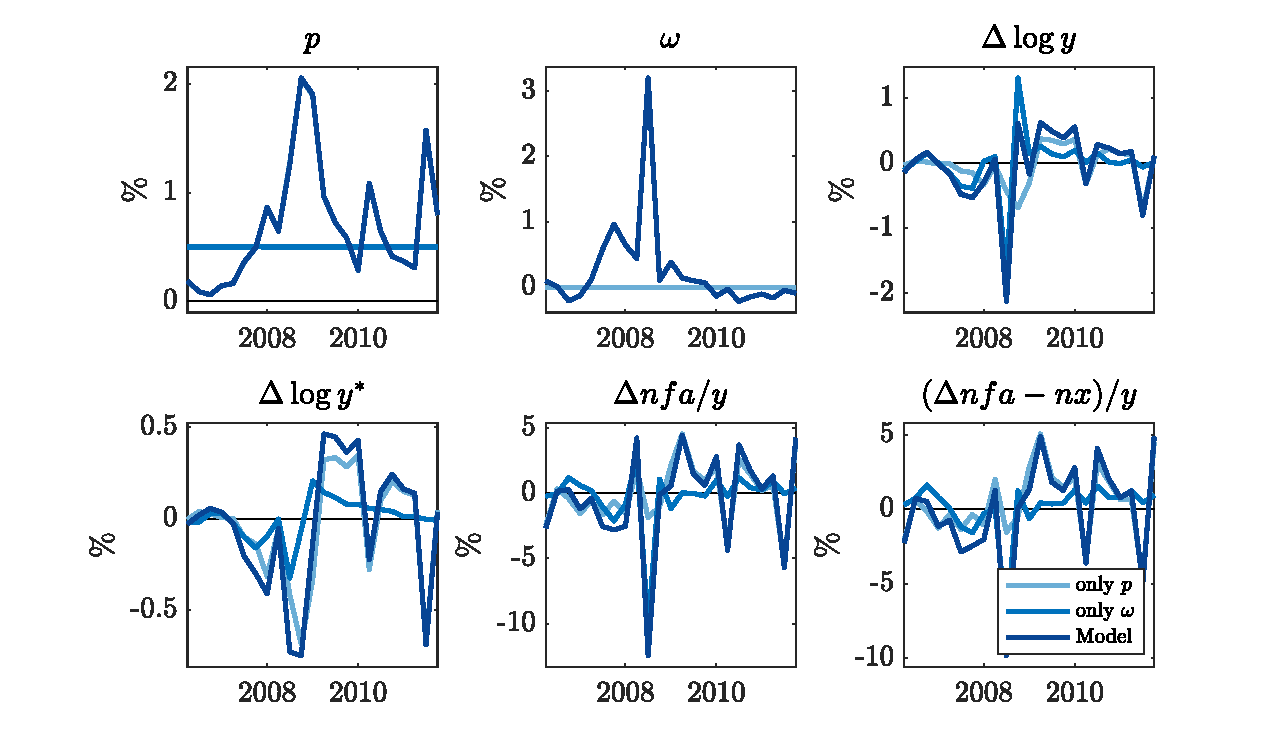
\includegraphics[width=\textwidth,clip=true,trim=0 0 0 0]{../output/figures/fig_6}
\renewcommand\thefigure{6}
\caption{simulation using observed $p$ and $\omega$ series}
\floatfoot{Notes: see notes to Figure \ref{fig:gr}.}
\end{figure}

\begin{figure}[H]
\centering
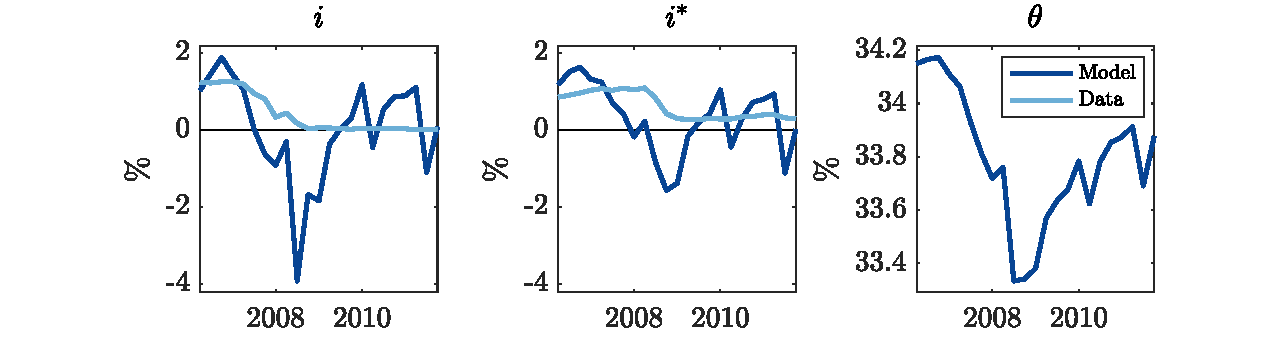
\includegraphics[width=\textwidth,clip=true,trim=0 0 0 0]{../output/figures/fig_7}
\renewcommand\thefigure{7}
\caption{simulation using observed $p$ and $\omega$ series}
\floatfoot{Notes: see notes to Figure \ref{fig:gr}.}
\end{figure}

\begin{figure}[H]
\centering
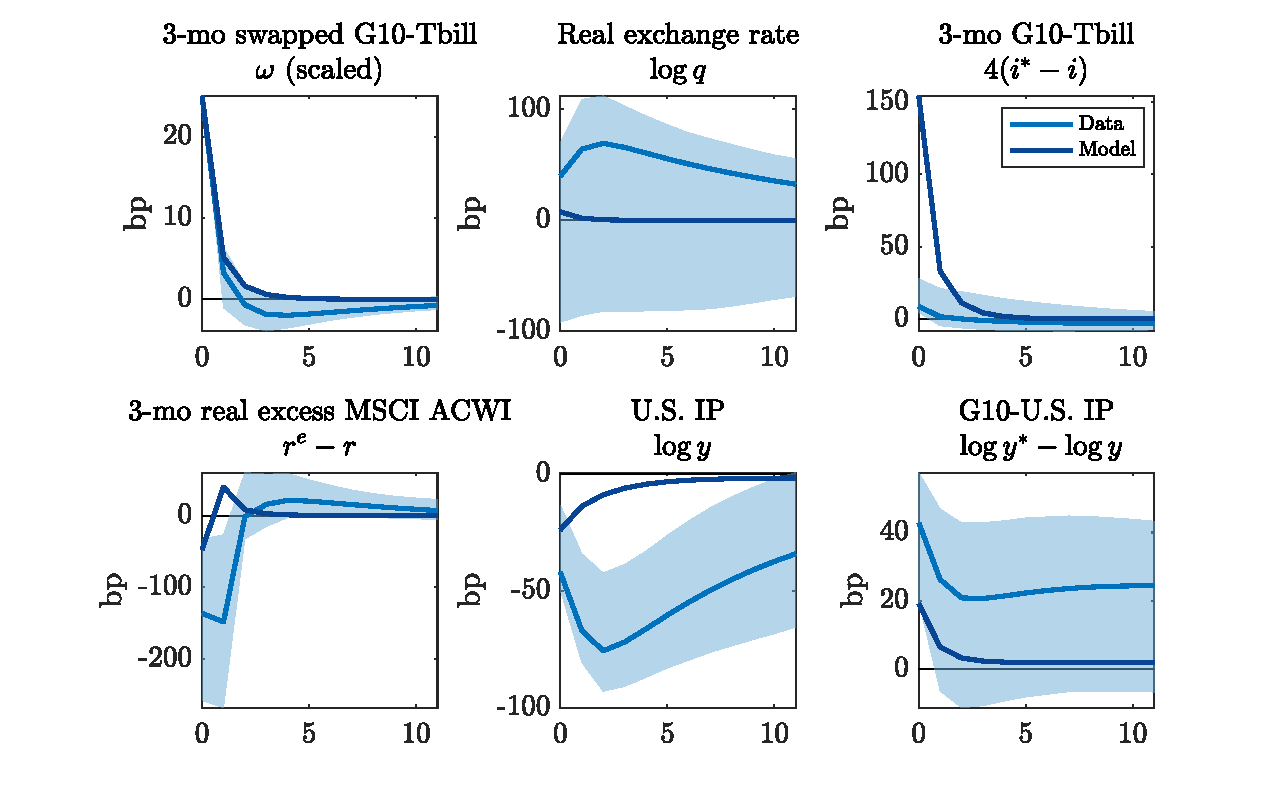
\includegraphics[width=1.0\textwidth,clip=true,trim=0 0 0 0]{../output/figures/fig_10}
\renewcommand\thefigure{9}
\caption{effects of safety shock in model and data}
\label{fig:safety_modelvsdata}
\floatfoot{Notes: in data, impulse responses estimated as in Figure \ref{fig:rvaremp} except using quarterly data over Q1 1995 -- Q4 2019.  In model, innovation to $\omega_t$ equals estimated innovation in swapped G10/Tbill spread, multiplied by ratio of unconditional volatilities of $\omega_t$ in model to swapped G10/Tbill spread in data.}
\end{figure}


\pagebreak

\begin{figure}[H]
\centering
\hspace*{-4cm}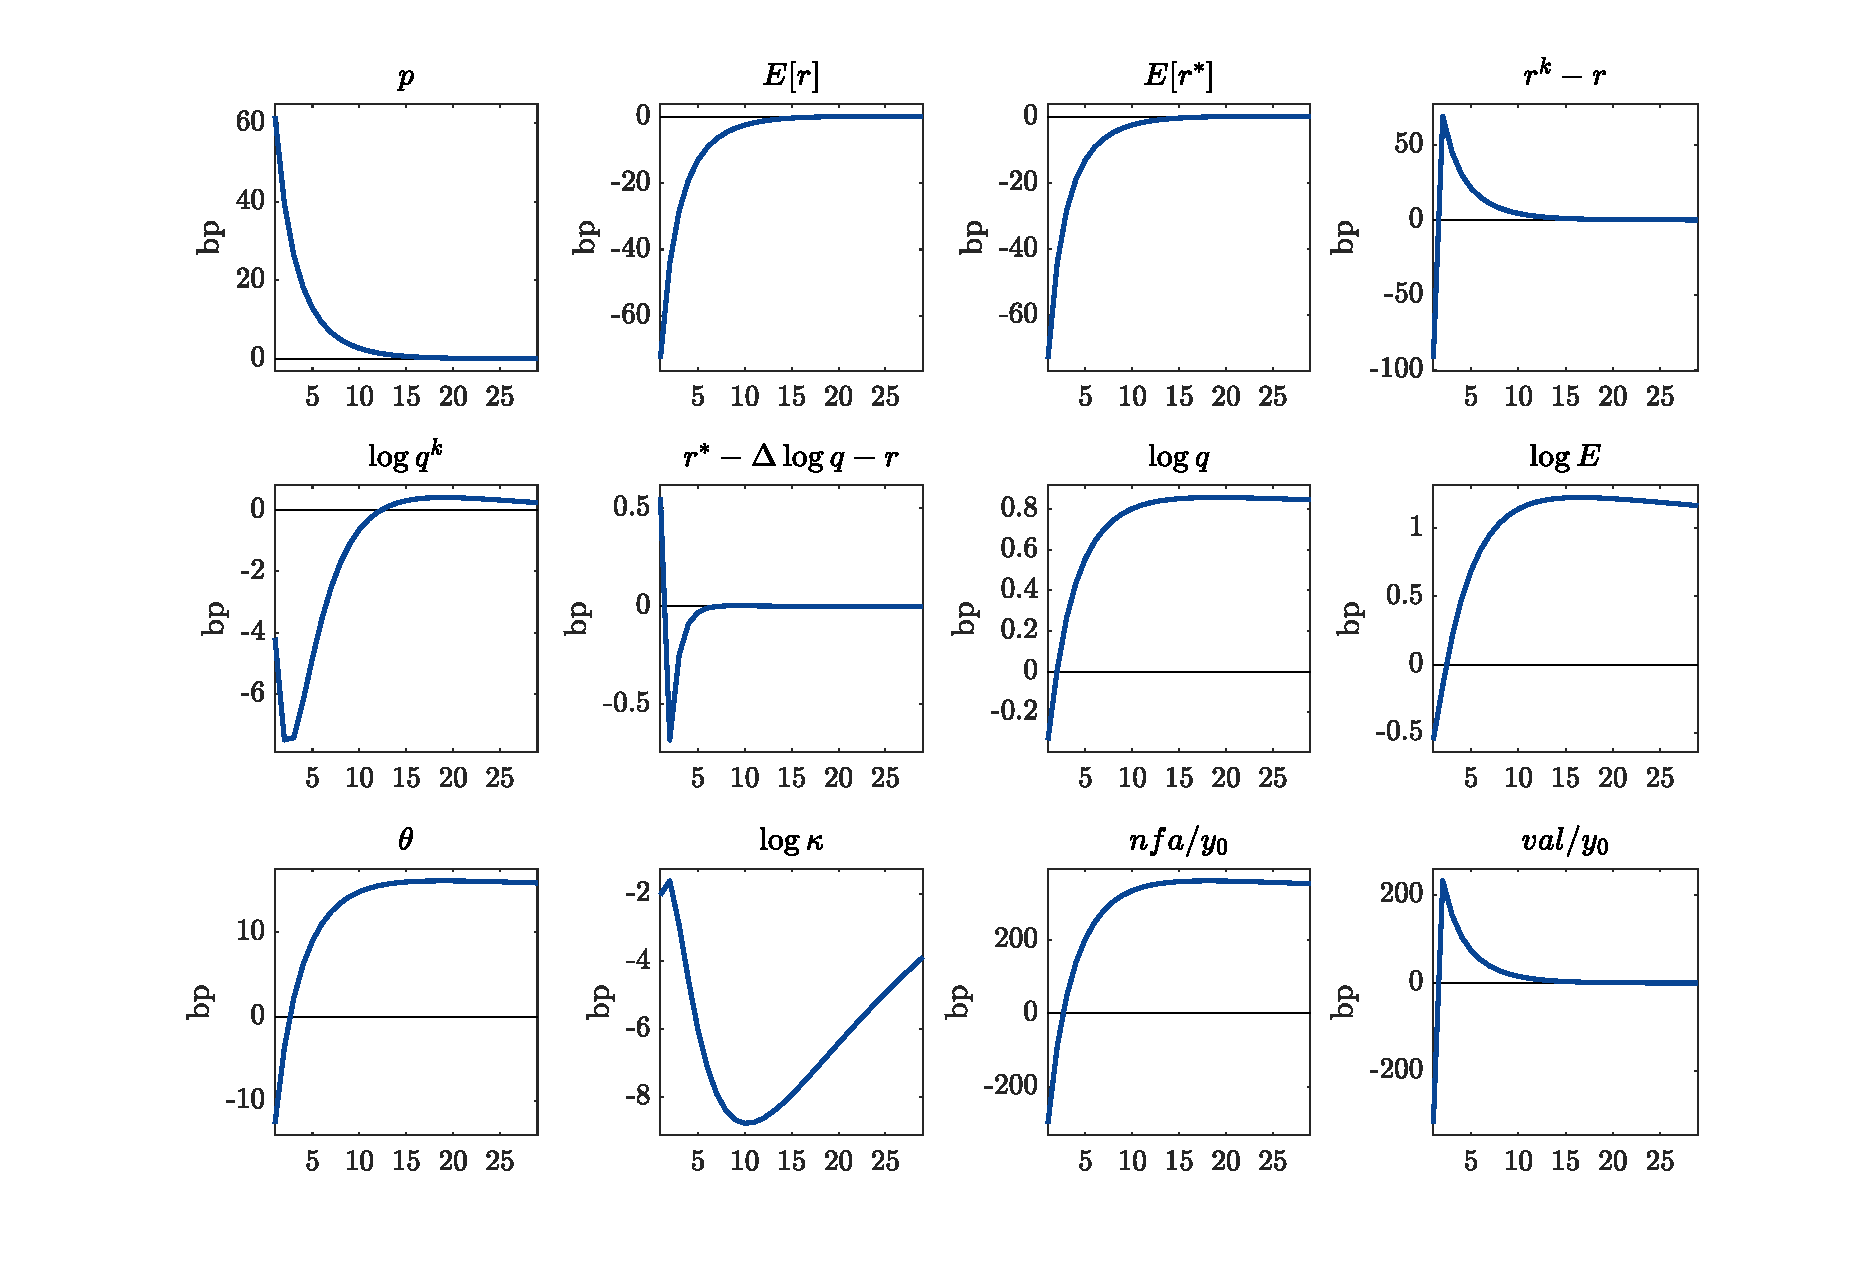
\includegraphics[width=1.5\textwidth,clip=true,trim=0 0 0 0]{../output/figures/fig_11}
\renewcommand\thefigure{10}
\caption{effects of increase in disaster probability - 1/2}
\floatfoot{Notes: impulse responses are average responses starting from 100 points drawn from ergodic distribution as described in note to Table \ref{tab:cal}.}
\end{figure}

\begin{figure}[H]
\centering
\hspace*{-4cm}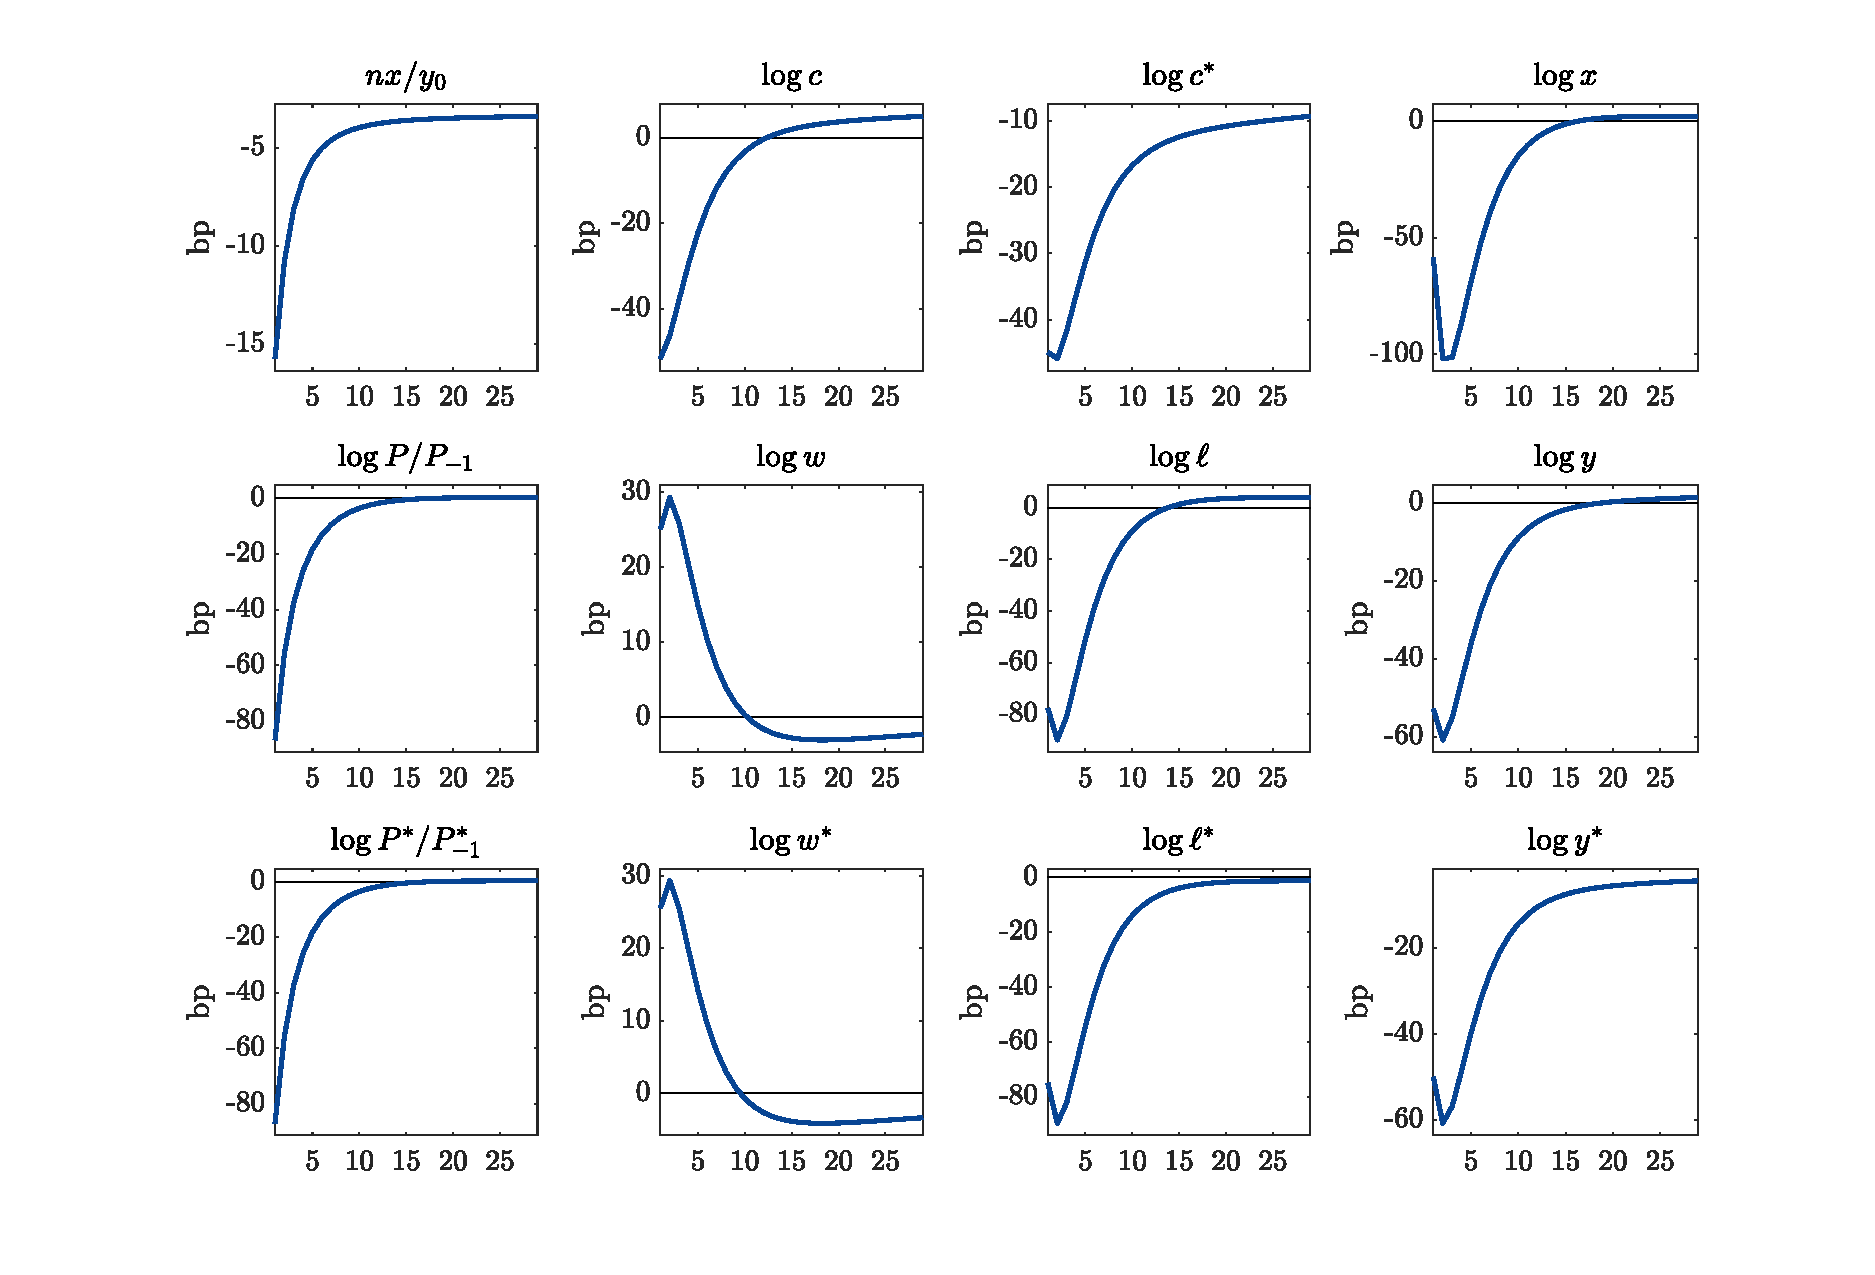
\includegraphics[width=1.5\textwidth,clip=true,trim=0 0 0 0]{../output/figures/fig_12}
\renewcommand\thefigure{11}
\caption{effects of increase in disaster probability - 2/2}
\floatfoot{Notes: impulse responses are average responses starting from 100 points drawn from ergodic distribution as described in note to Table \ref{tab:cal}.}
\end{figure}

\begin{figure}[H]
\centering
\hspace*{-4cm}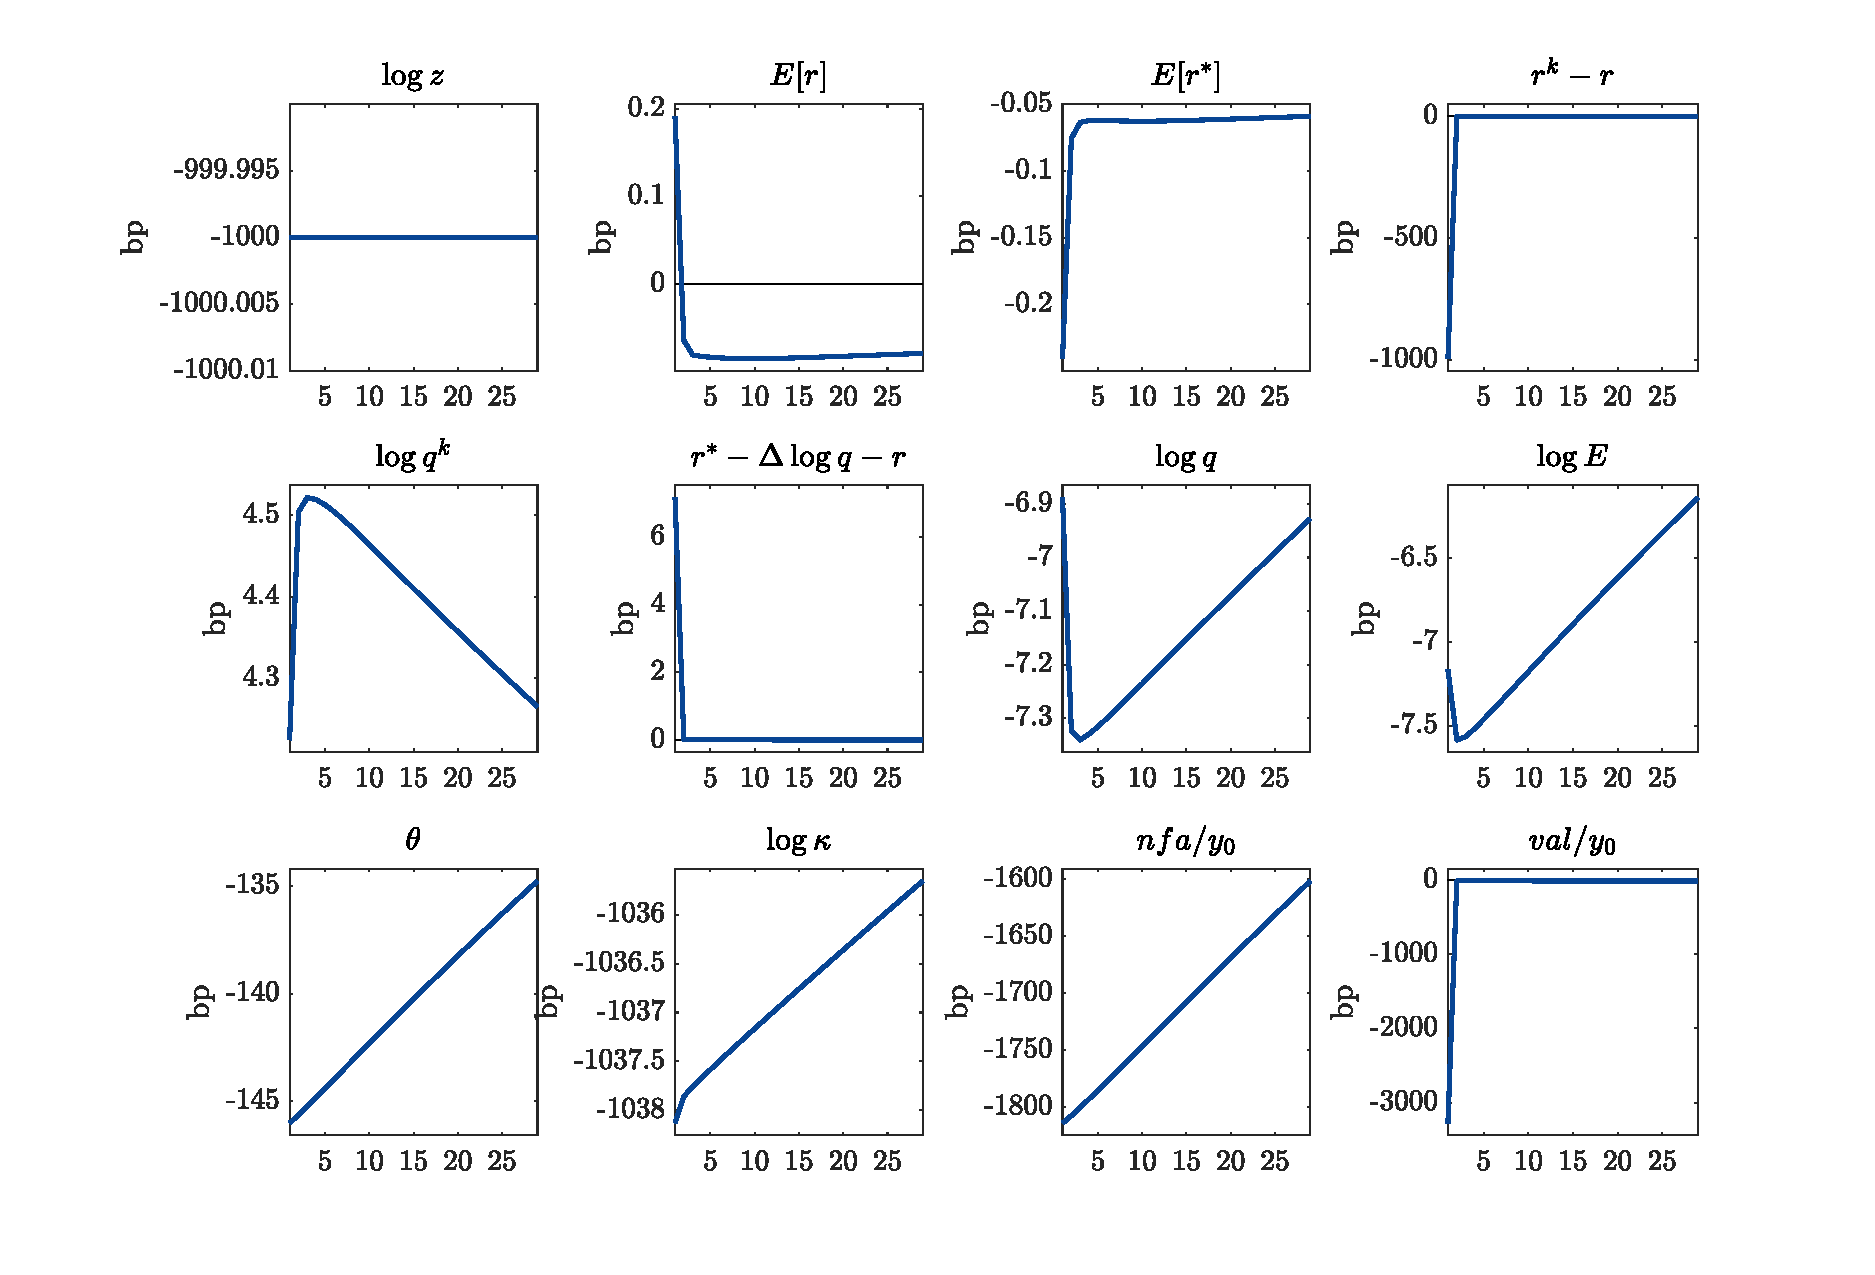
\includegraphics[width=1.5\textwidth,clip=true,trim=0 0 0 0]{../output/figures/fig_13}
\renewcommand\thefigure{12}
\caption{effects of disaster realization - 1/2}
\floatfoot{Notes: impulse responses are average responses starting from 100 points drawn from ergodic distribution as described in note to Table \ref{tab:cal}.}
\end{figure}

\begin{figure}[H]
\centering
\hspace*{-4cm}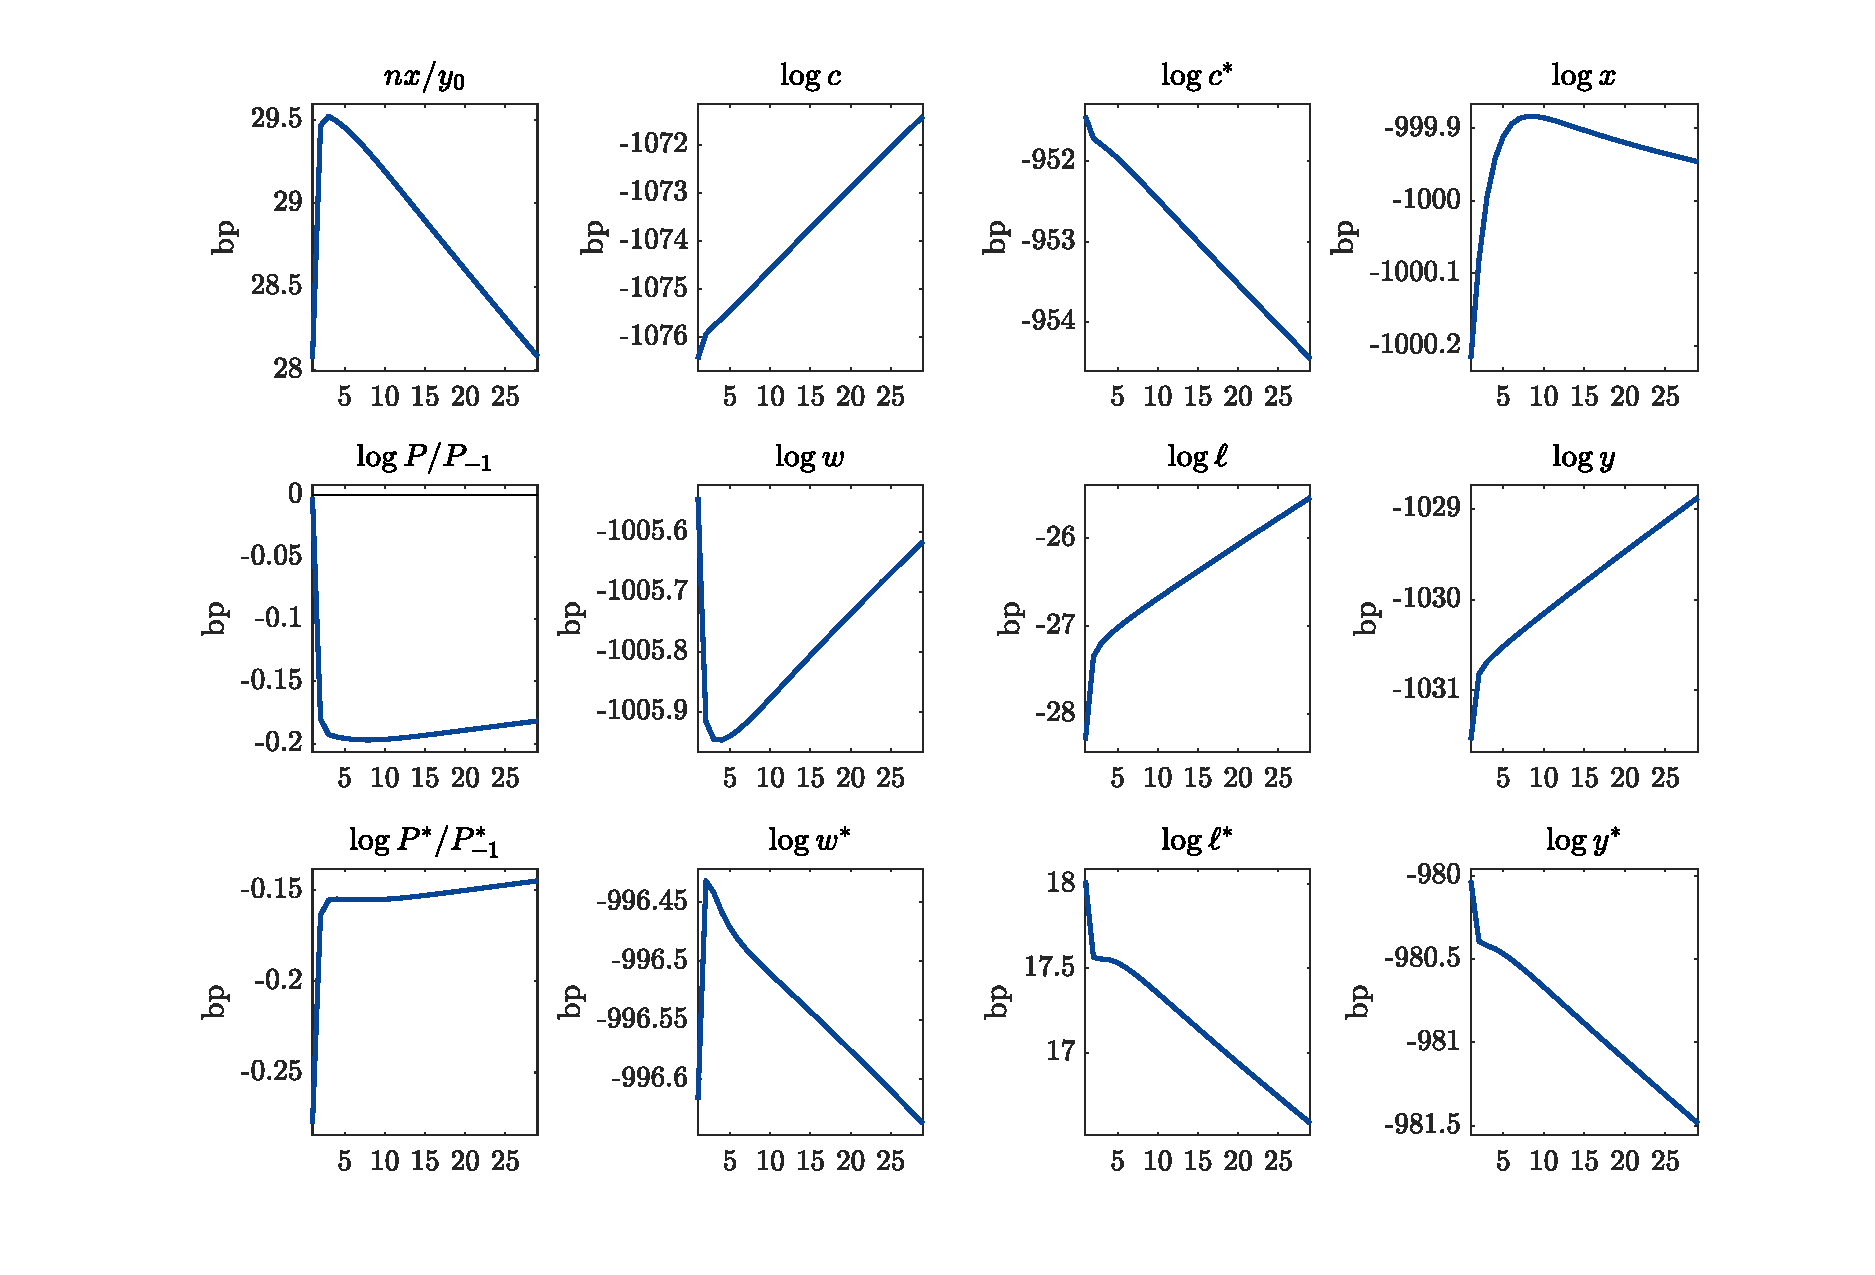
\includegraphics[width=1.5\textwidth,clip=true,trim=0 0 0 0]{../output/figures/fig_14}
\renewcommand\thefigure{13}
\caption{effects of disaster realization - 2/2}
\floatfoot{Notes: impulse responses are average responses starting from 100 points drawn from ergodic distribution as described in note to Table \ref{tab:cal}.}
\end{figure}

\begin{figure}[H]
\centering
\hspace*{-4cm}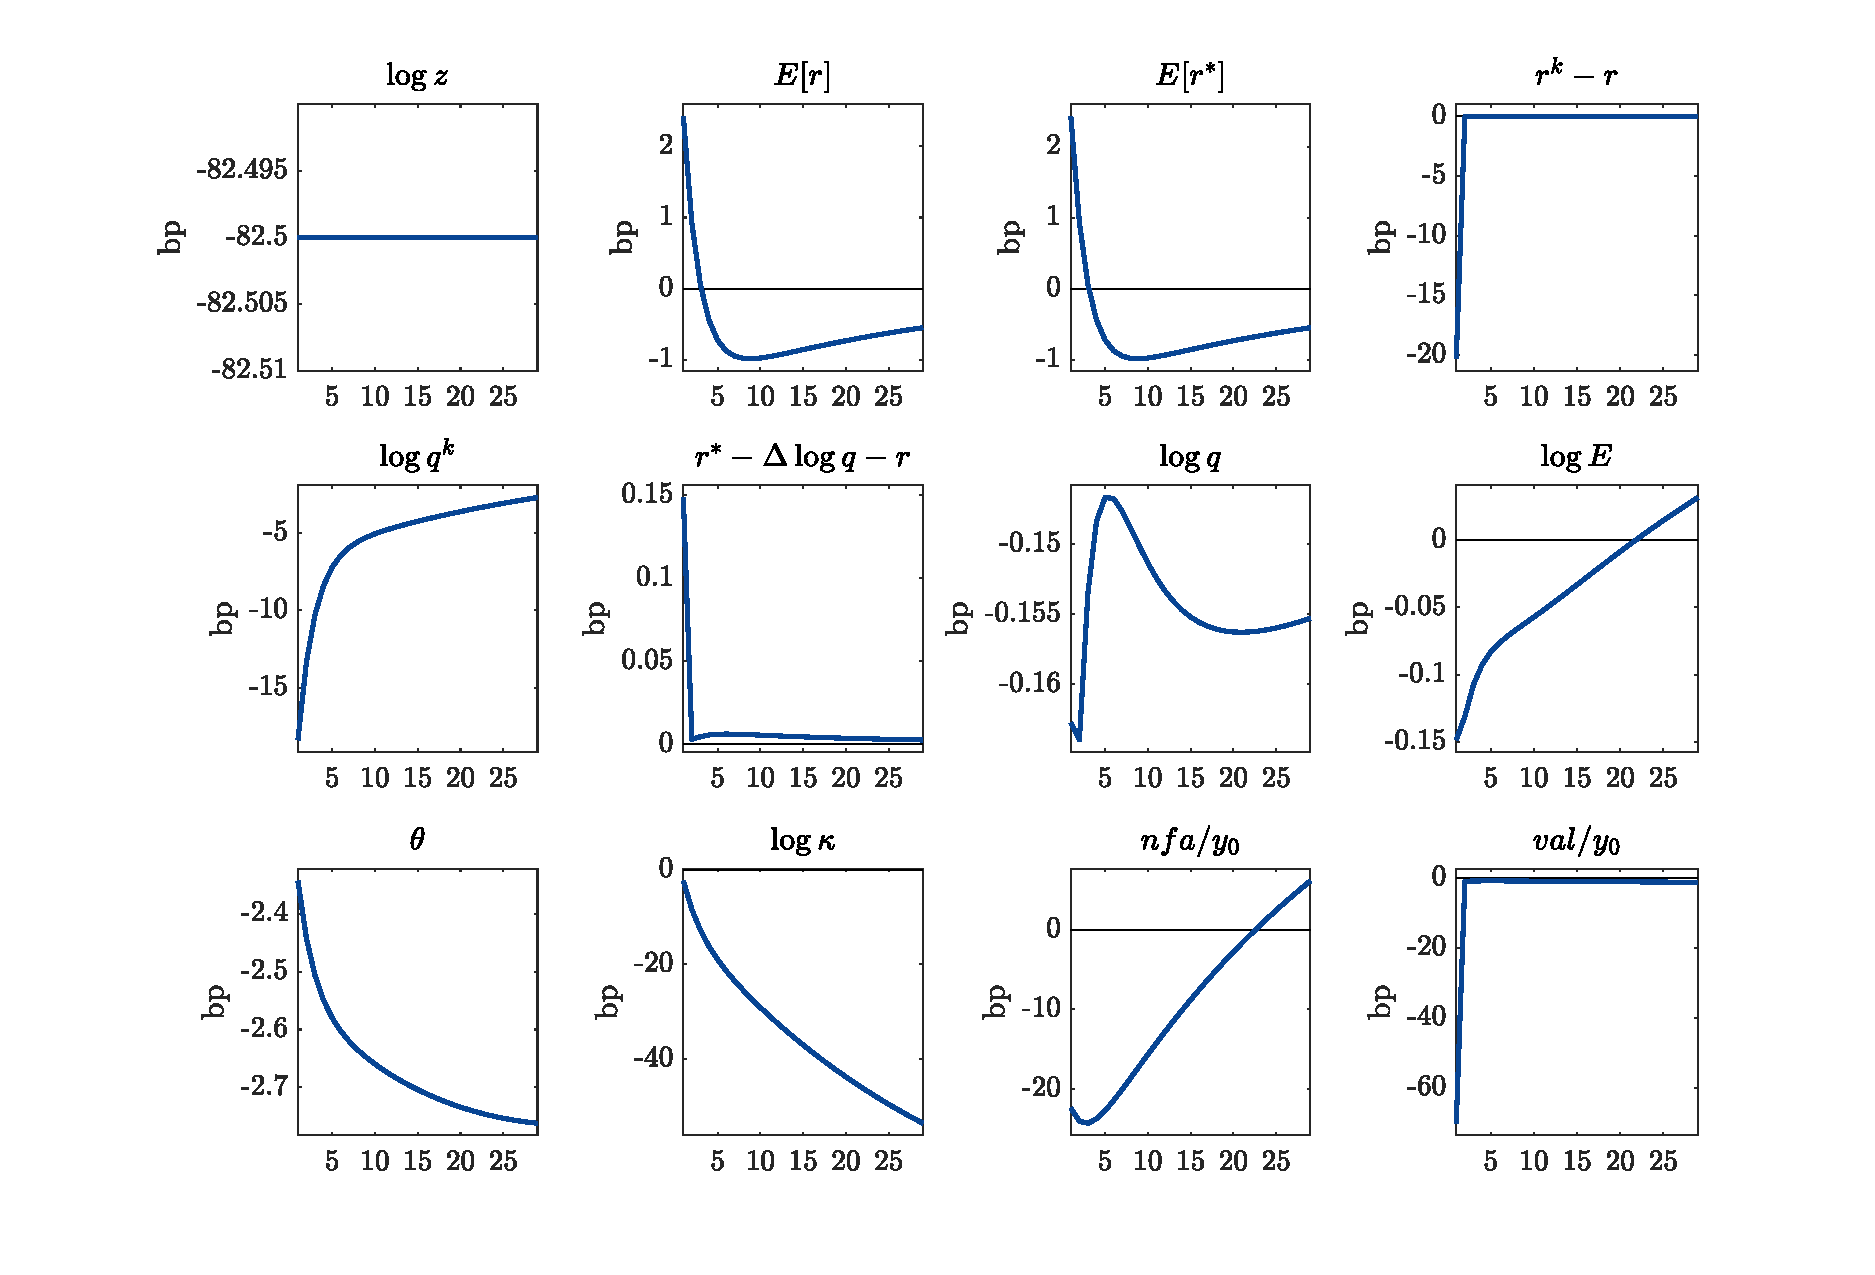
\includegraphics[width=1.5\textwidth,clip=true,trim=0 0 0 0]{../output/figures/fig_15}
\renewcommand\thefigure{14}
\caption{effects of global productivity shock - 1/2}
\floatfoot{Notes: impulse responses are average responses starting from 100 points drawn from ergodic distribution as described in note to Table \ref{tab:cal}.}
\end{figure}

\begin{figure}[H]
\centering
\hspace*{-4cm}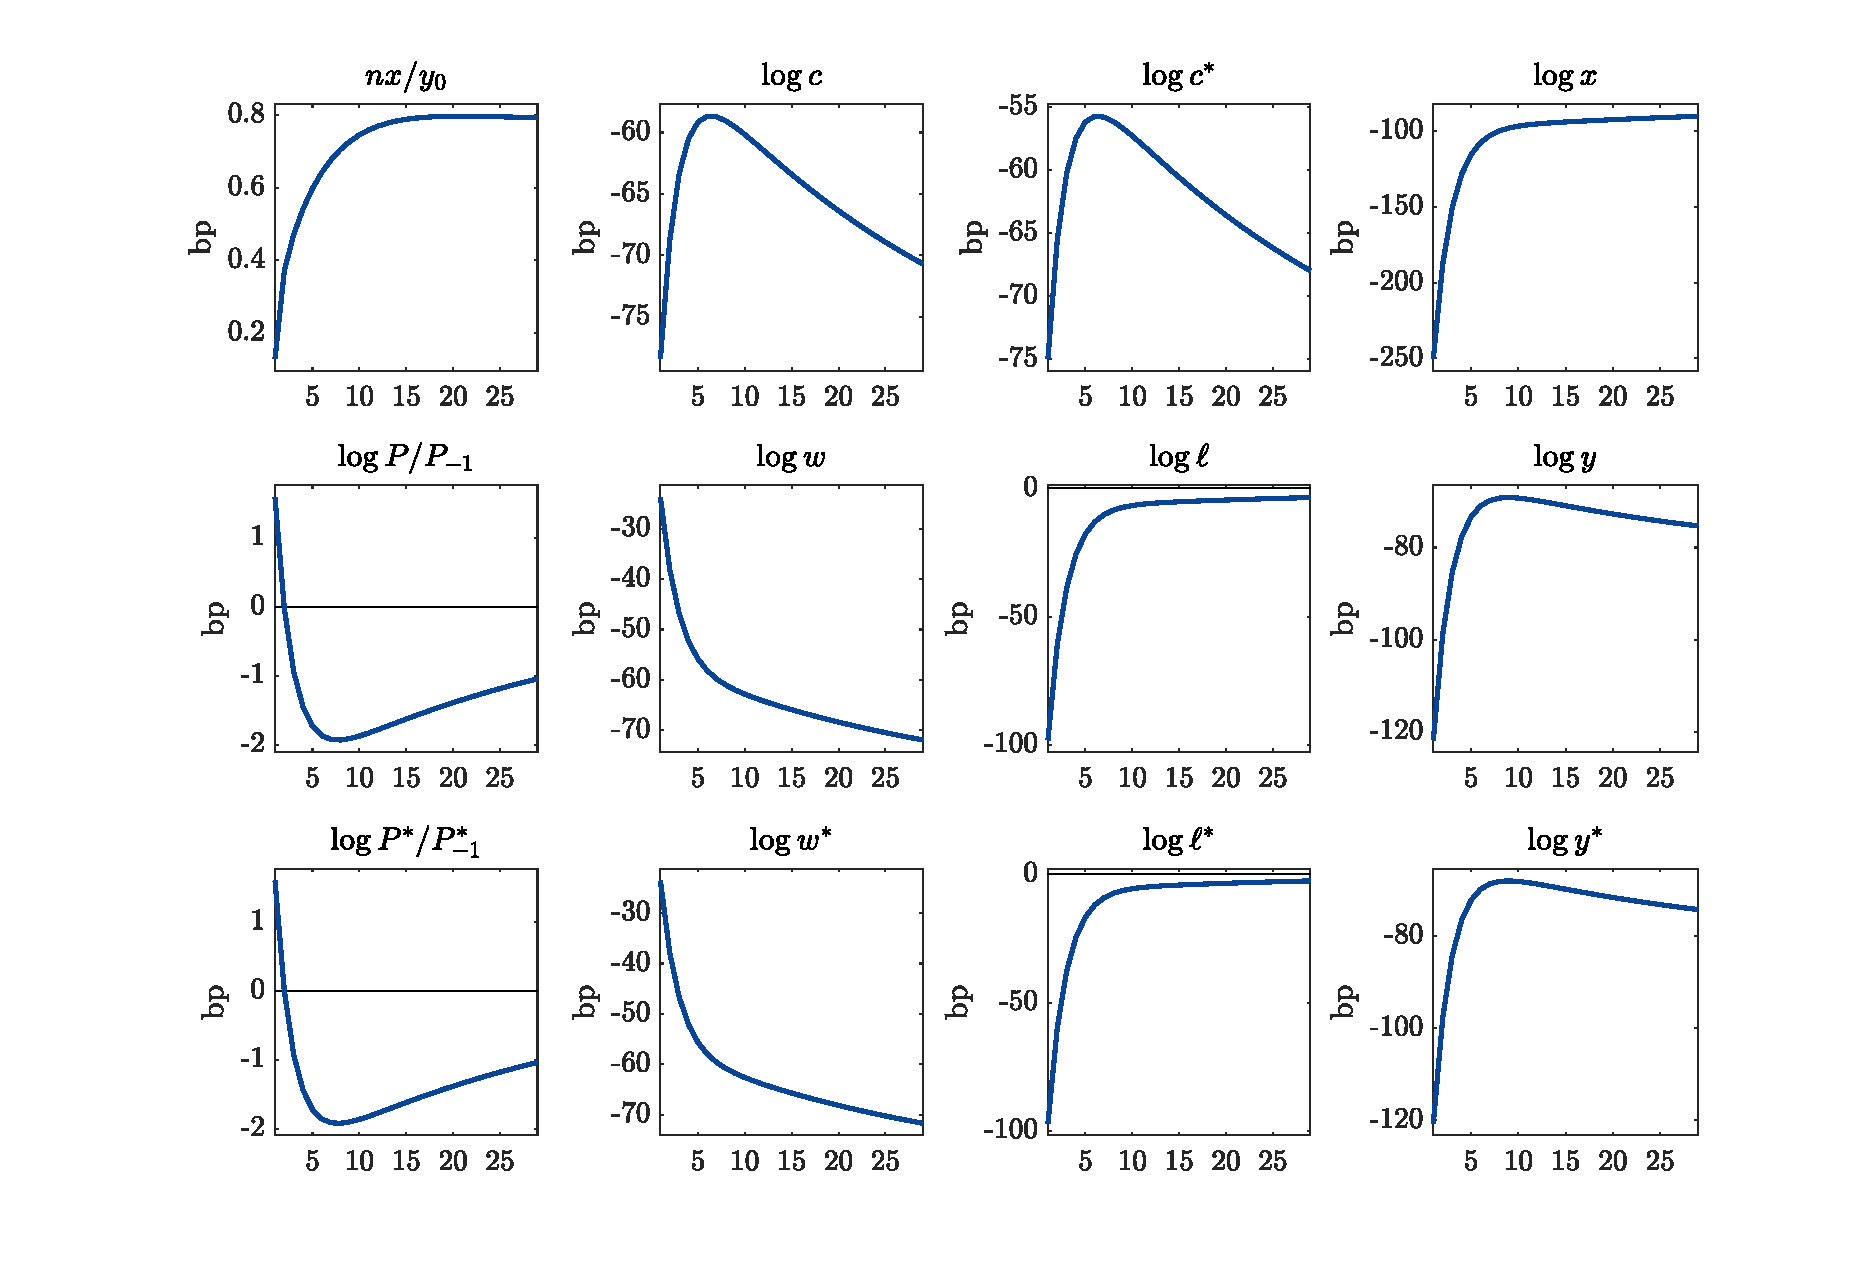
\includegraphics[width=1.5\textwidth,clip=true,trim=0 0 0 0]{../output/figures/fig_16}
\renewcommand\thefigure{15}
\caption{effects of global productivity shock - 2/2}
\floatfoot{Notes: impulse responses are average responses starting from 100 points drawn from ergodic distribution as described in note to Table \ref{tab:cal}.}
\end{figure}

\begin{figure}[H]
\centering
\hspace*{-4cm}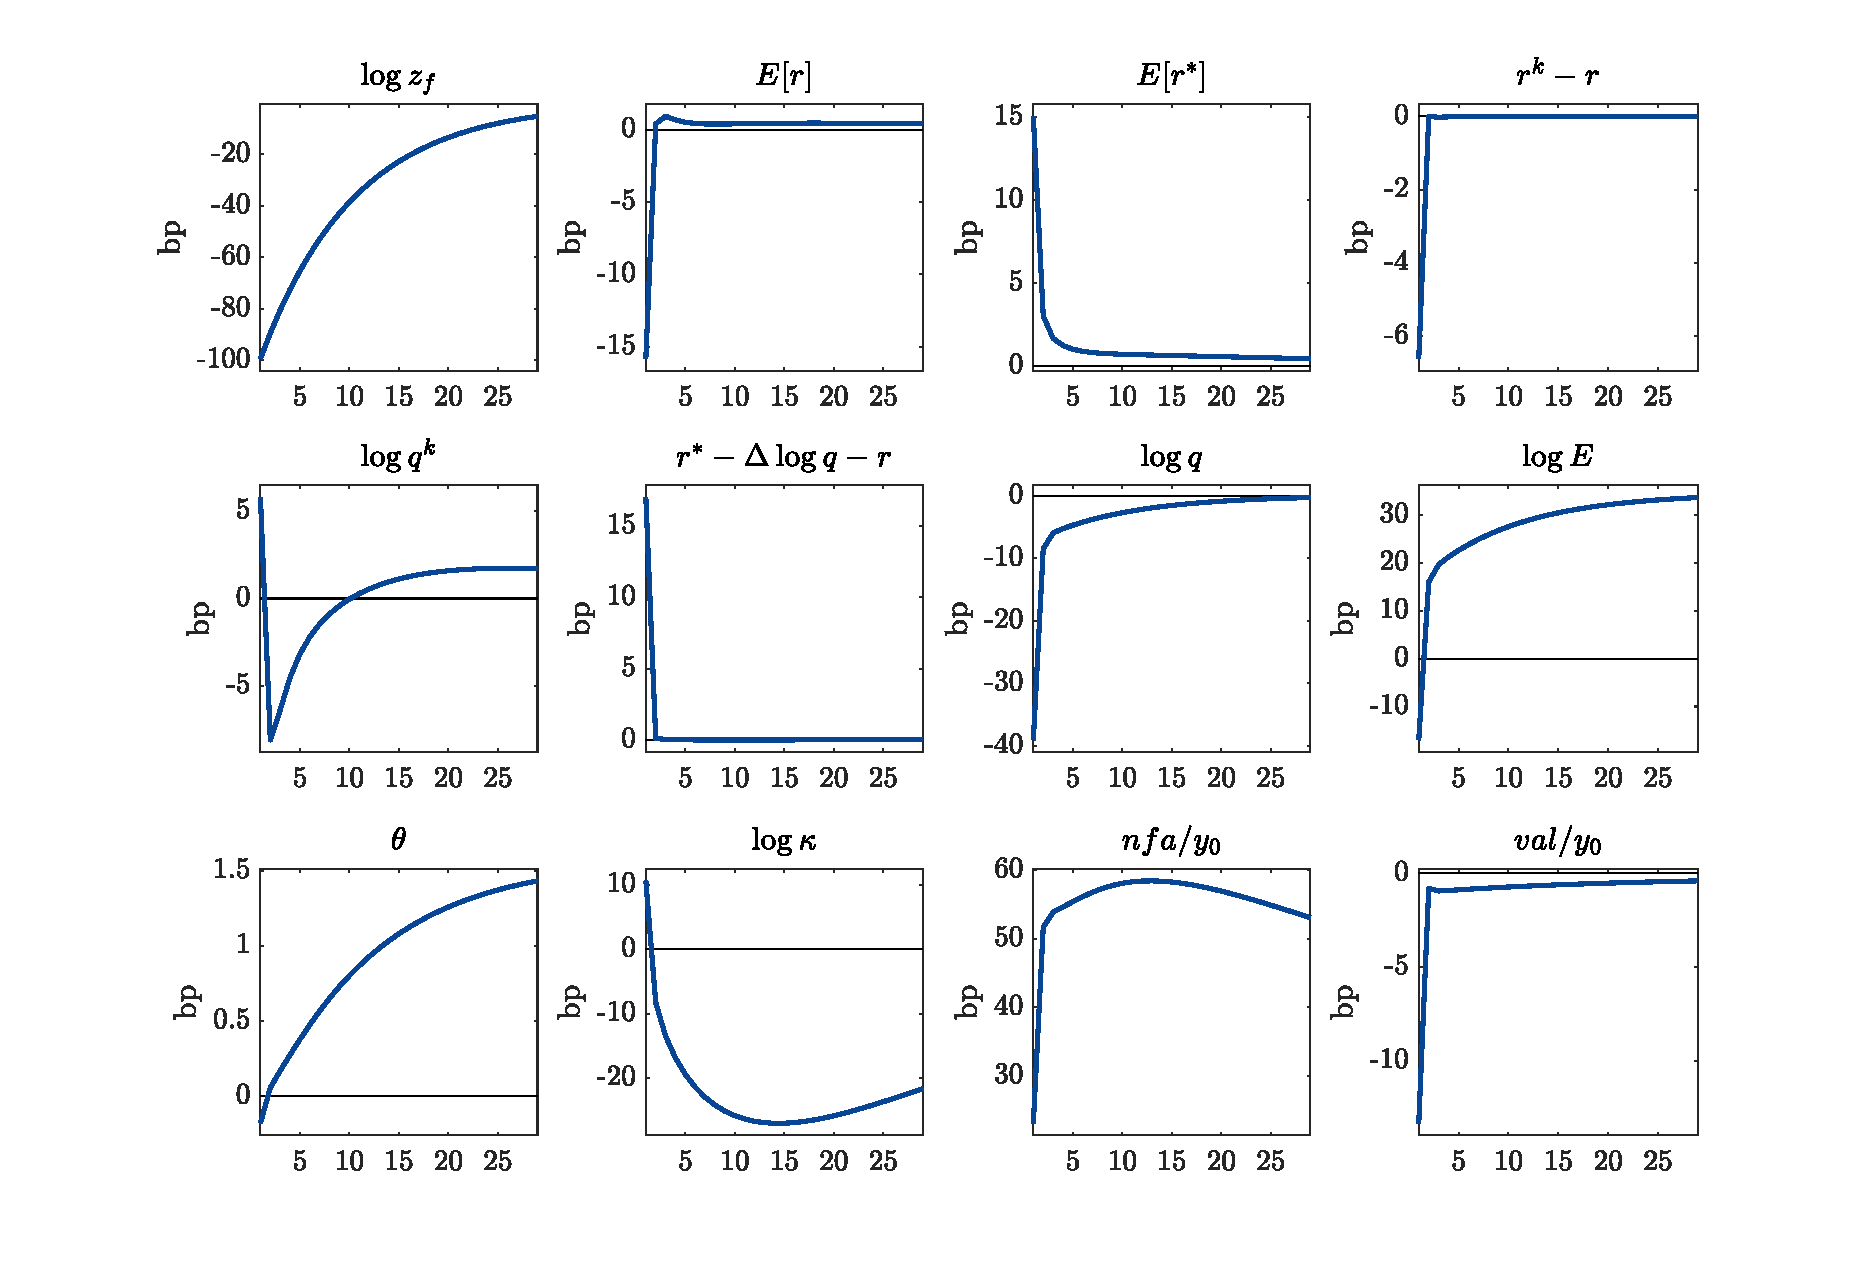
\includegraphics[width=1.5\textwidth,clip=true,trim=0 0 0 0]{../output/figures/fig_17}
\renewcommand\thefigure{16}
\caption{effects of relative productivity shock - 1/2}
\floatfoot{Notes: impulse responses are average responses starting from 100 points drawn from ergodic distribution as described in note to Table \ref{tab:cal}.}
\end{figure}

\begin{figure}[H]
\centering
\hspace*{-4cm}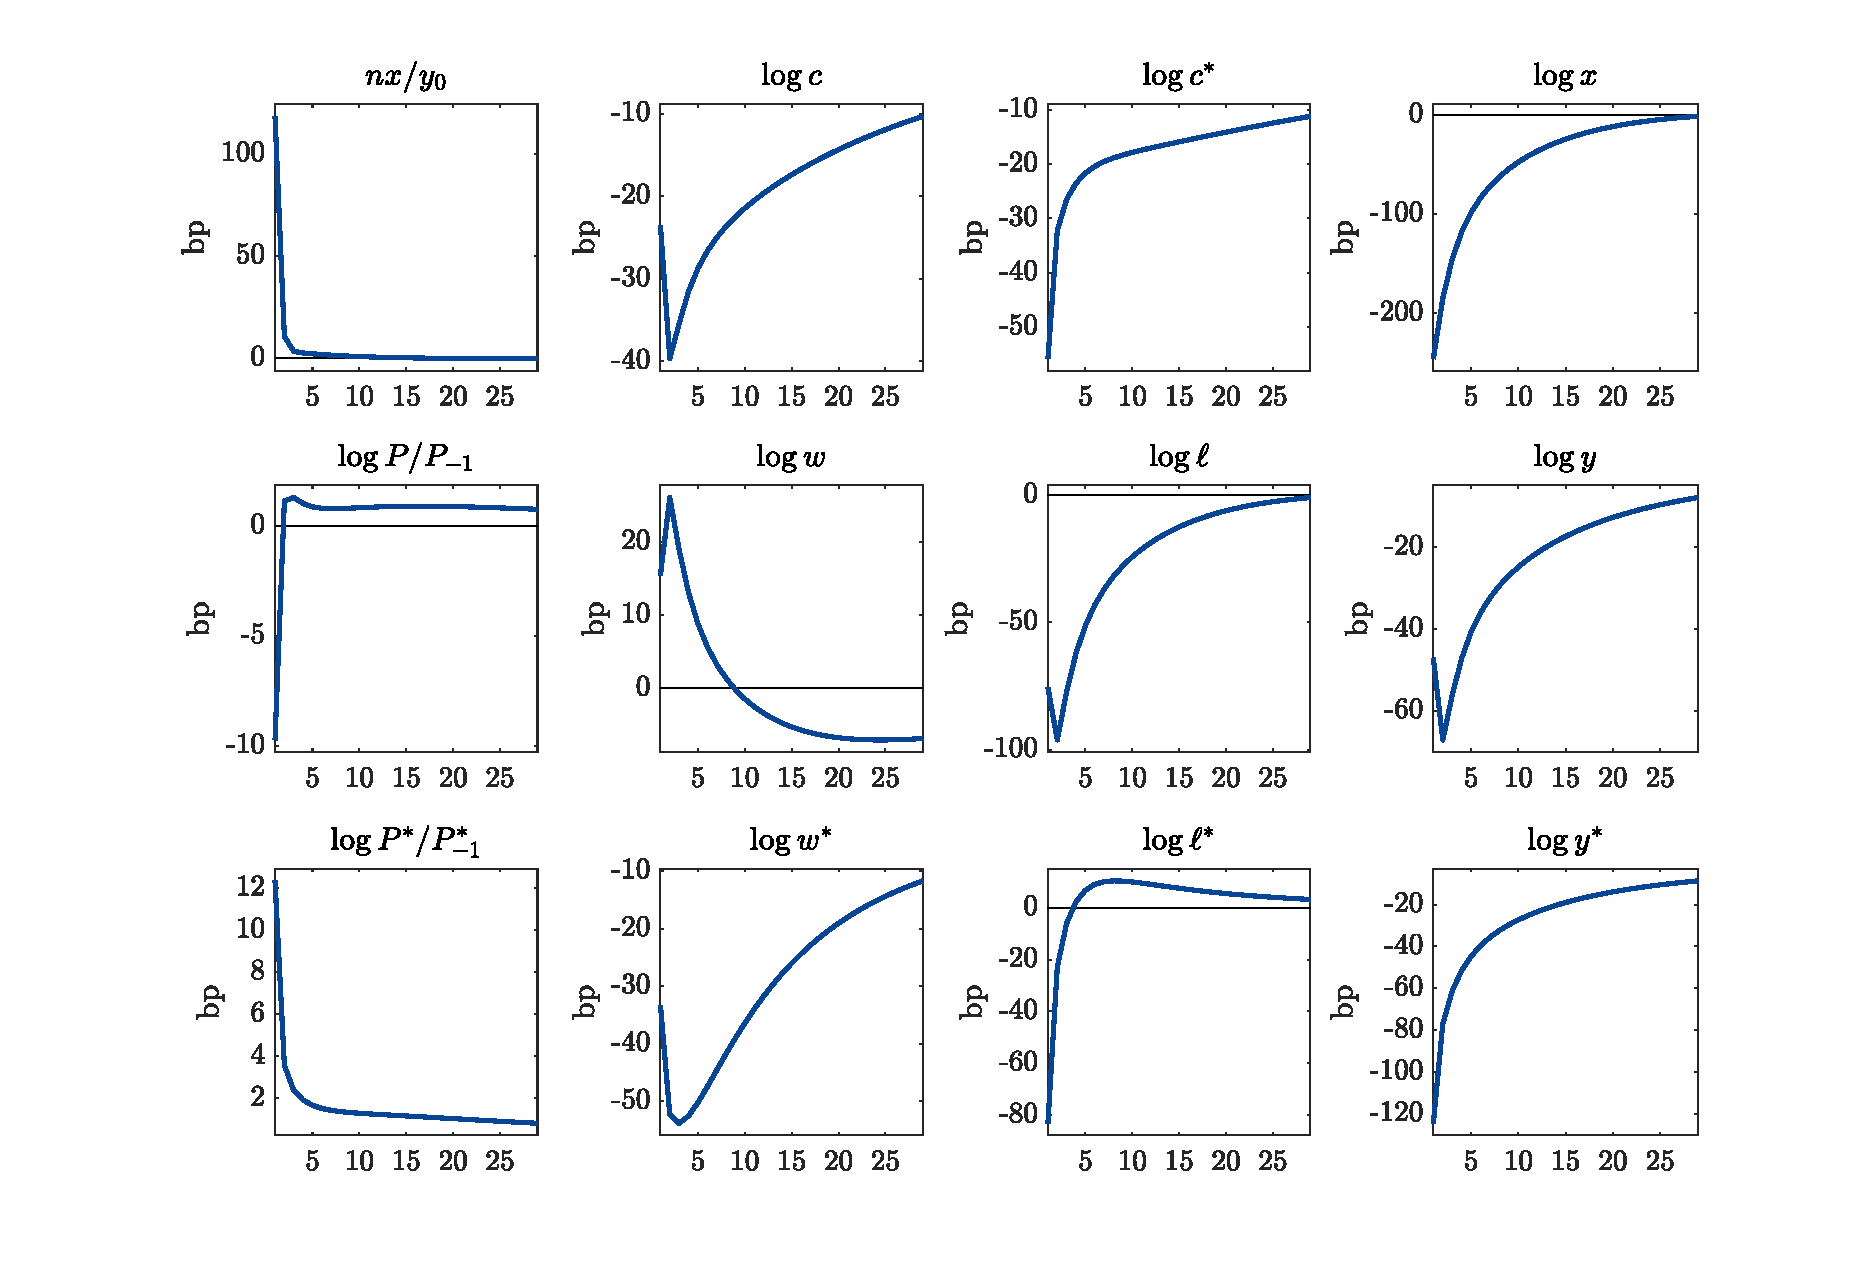
\includegraphics[width=1.5\textwidth,clip=true,trim=0 0 0 0]{../output/figures/fig_18}
\renewcommand\thefigure{17}
\caption{effects of relative productivity shock - 2/2}
\floatfoot{Notes: impulse responses are average responses starting from 100 points drawn from ergodic distribution as described in note to Table \ref{tab:cal}.}
\end{figure}

\begin{figure}[H]
\centering
\hspace*{-4cm}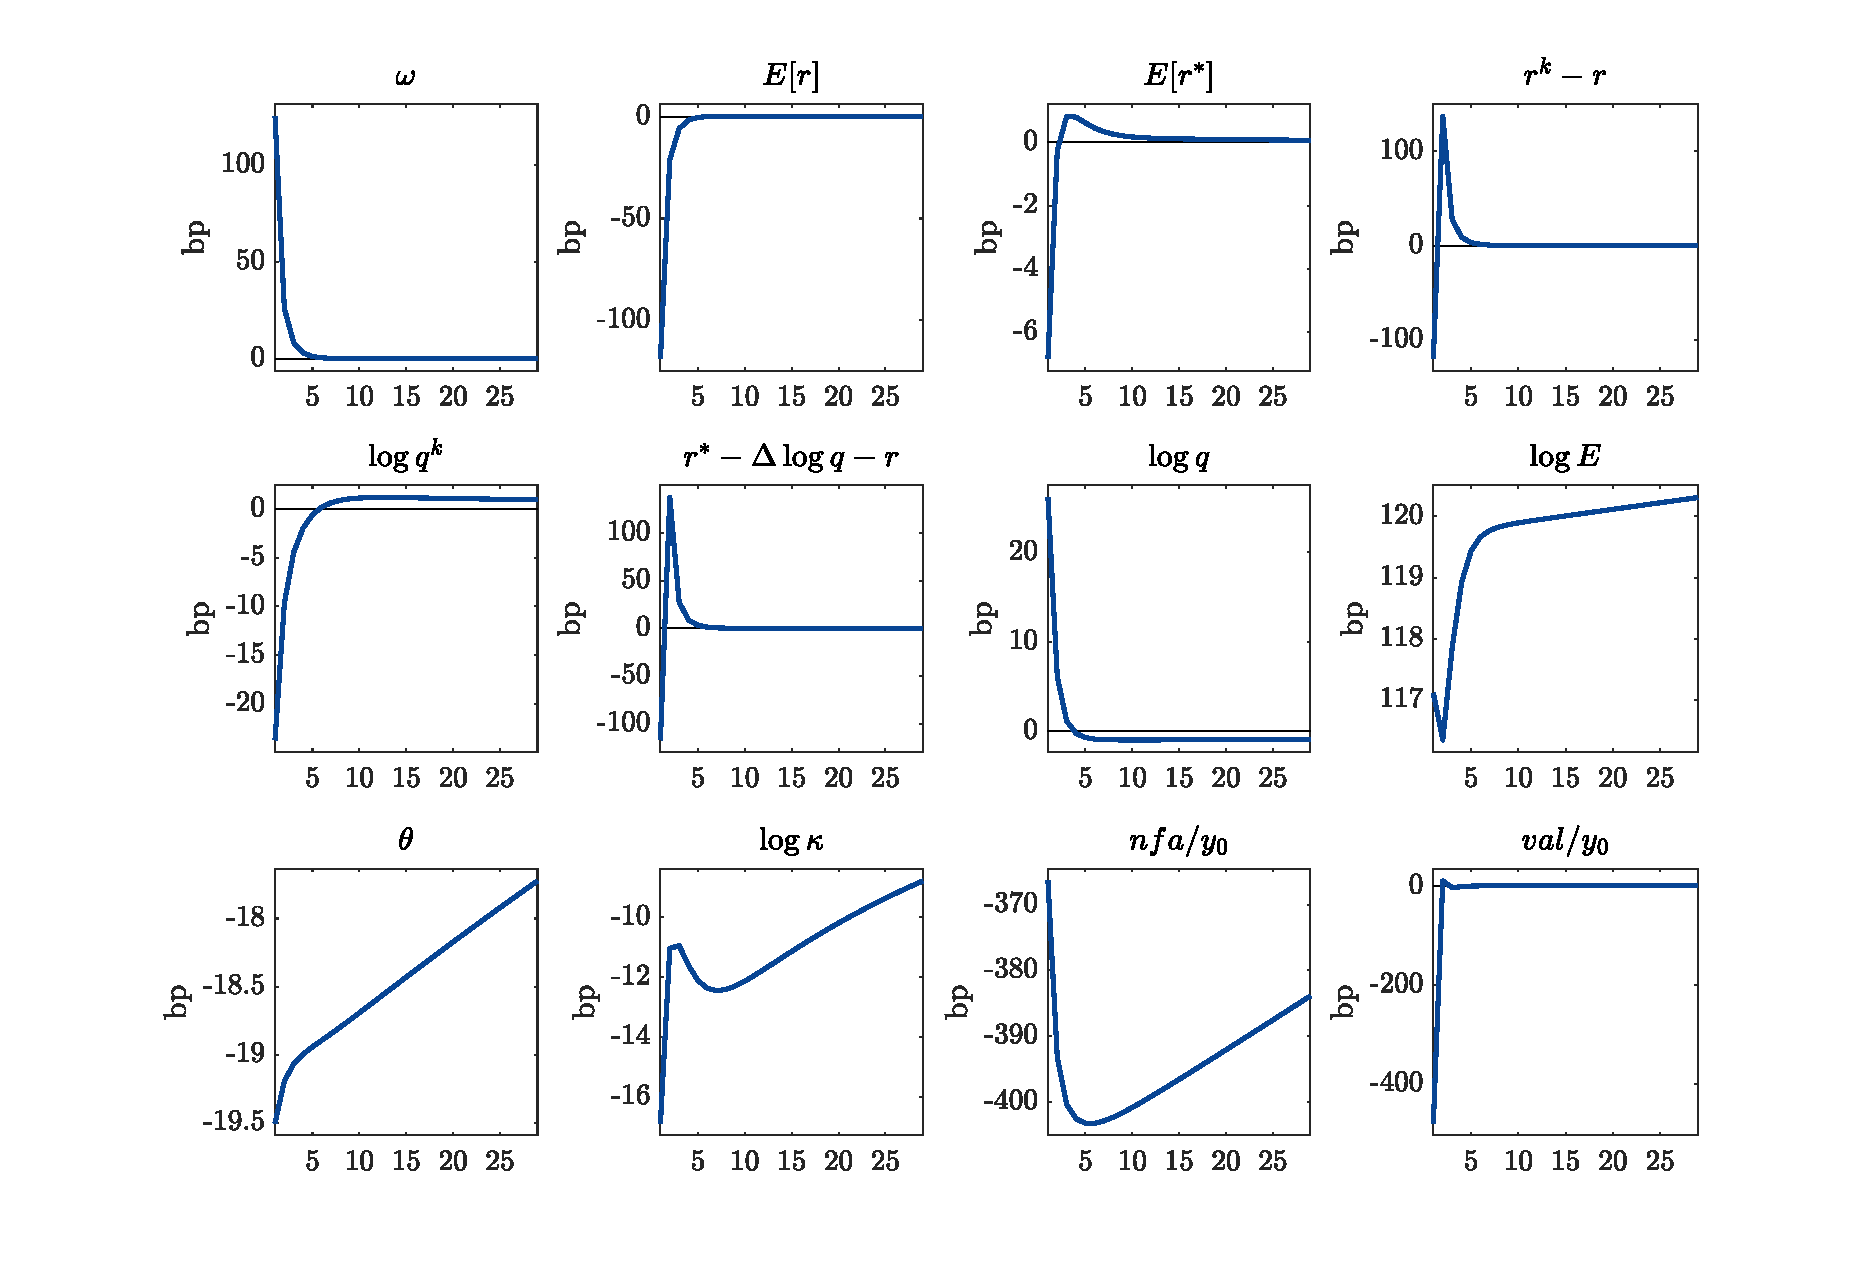
\includegraphics[width=1.5\textwidth,clip=true,trim=0 0 0 0]{../output/figures/fig_19}
\renewcommand\thefigure{18}
\caption{effects of safety shock - 1/2}
\floatfoot{Notes: impulse responses are average responses starting from 100 points drawn from ergodic distribution as described in note to Table \ref{tab:cal}.}
\end{figure}

\begin{figure}[H]
\centering
\hspace*{-4cm}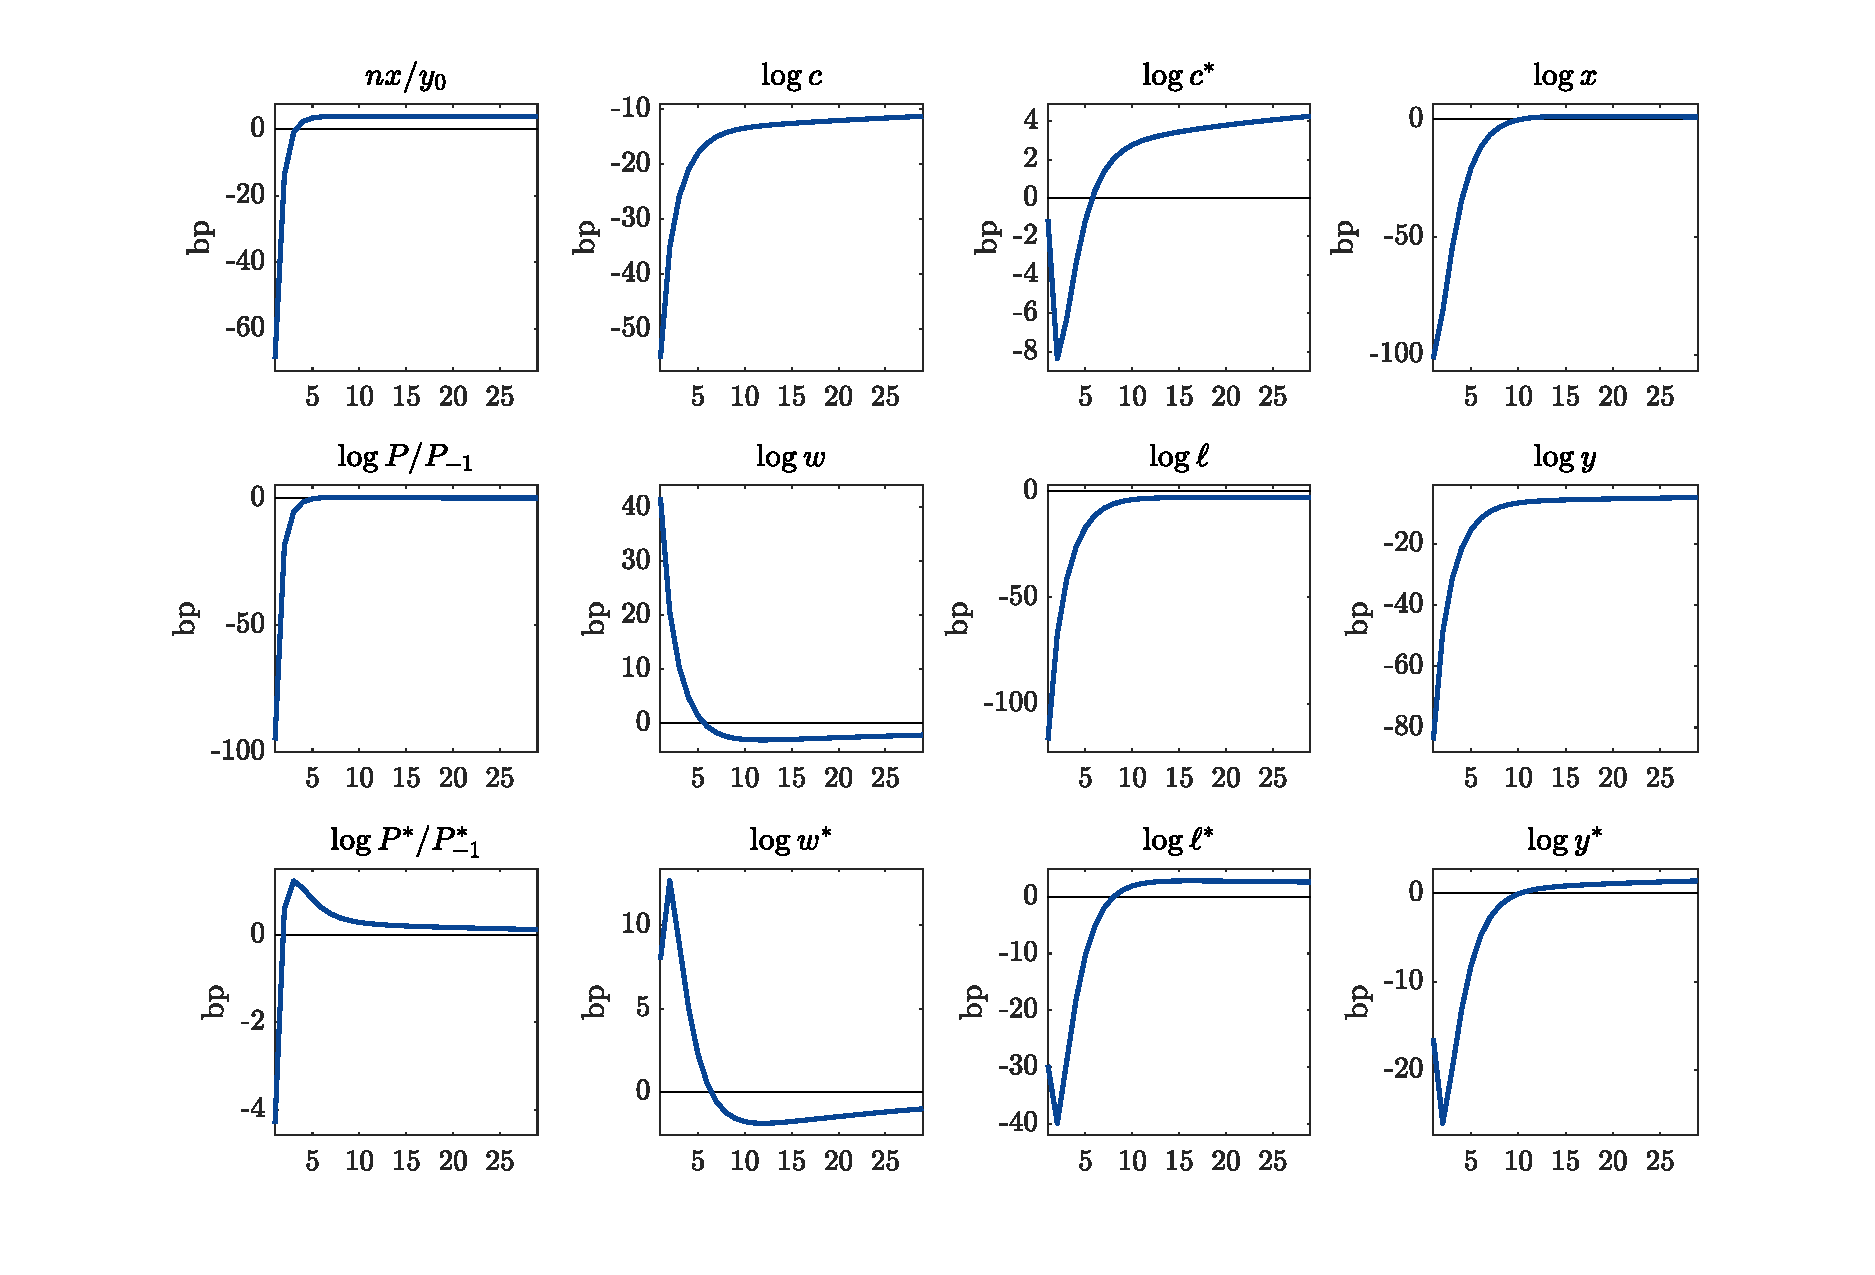
\includegraphics[width=1.5\textwidth,clip=true,trim=0 0 0 0]{../output/figures/fig_20}
\renewcommand\thefigure{19}
\caption{effects of safety shock - 2/2}
\floatfoot{Notes: impulse responses are average responses starting from 100 points drawn from ergodic distribution as described in note to Table \ref{tab:cal}.}
\end{figure}

\section{Additional results}

\begin{table}[H]
\centering
\bgroup
\def\arraystretch{1.25}
\begin{tabular}{l|cc} \hline
 \emph{Q3 07 - Q3 09} & Data & Model \\ \hline 
$\Delta \log y$ &    -4.7536\% &    -1.3304\%  \\ 
$\Delta \log y^*$ &    -5.1183\% &    -1.4699\%  \\ 
$\Delta nfa/y$ &   -10.0397\% &    -8.6086\%  \\  \hline 

\end{tabular}
\egroup
\renewcommand\thetable{A1}
\caption{Output decline}
\end{table}

\begin{table}[H]
\centering
\bgroup
\def\arraystretch{1.25}
\begin{tabular}{l|ccc} \hline
  & Model  & No $\omega$ & $\gamma=\gamma^\ast$ \\ \hline 
\emph{As share of} $Var\left((\mathbb{E}_t - \mathbb{E}_{t-1})nfa_t\right)$: & & \\$Cov\left(-(\mathbb{E}_t - \mathbb{E}_{t-1})\sum_{h=1}^{500} \left(\prod_{i=1}^{h} \frac{1}{1+r_{t+i}^k}\right)nx_{t+h},(\mathbb{E}_t - \mathbb{E}_{t-1})nfa_t\right)$ & $  32.3\%$ & $  76.2\%$ & $  99.1\%$ \\ 
$Cov\left(-(\mathbb{E}_t - \mathbb{E}_{t-1})\sum_{h=1}^{500} \left(\prod_{i=1}^{h} \frac{1}{1+r_{t+i}^k}\right)val_{t+h},(\mathbb{E}_t - \mathbb{E}_{t-1})nfa_t\right)$ & $  67.6\%$ & $  23.8\%$ & $   0.9\%$ \\ 
$Cov\left(-(\mathbb{E}_t - \mathbb{E}_{t-1})\sum_{h=1}^{500} \left(\prod_{i=1}^{h} \frac{1}{1+r_{t+i}^k}\right)val^r_{t+h},(\mathbb{E}_t - \mathbb{E}_{t-1})nfa_t\right)$ & $  67.0\%$ & $  23.4\%$ & $  -0.1\%$ \\ 
$Cov\left(-(\mathbb{E}_t - \mathbb{E}_{t-1})\sum_{h=1}^{500} \left(\prod_{i=1}^{h} \frac{1}{1+r_{t+i}^k}\right)val^{r^\ast}_{t+h},(\mathbb{E}_t - \mathbb{E}_{t-1})nfa_t\right)$ & $   0.3\%$ & $   0.4\%$ & $   0.1\%$ \\ 
$Cov\left(-(\mathbb{E}_t - \mathbb{E}_{t-1})\sum_{h=1}^{500} \left(\prod_{i=1}^{h} \frac{1}{1+r_{t+i}^k}\right)val^s_{t+h},(\mathbb{E}_t - \mathbb{E}_{t-1})nfa_t\right)$ & $   0.4\%$ & $   0.0\%$ & $   0.8\%$ \\ 
$Cov\left((\mathbb{E}_t - \mathbb{E}_{t-1})\left(\prod_{i=1500200} \frac{1}{1+r_{t+i}^k}\right)nfa_{t+500},(\mathbb{E}_t - \mathbb{E}_{t-1})nfa_t\right)$ & $   0.1\%$ & $   0.1\%$ & $  -0.0\%$ \\ 
\hline 

\end{tabular}
\egroup
\renewcommand\thetable{7}
\caption{understanding U.S. external adjustment}
\floatfoot{Notes: moments are computed as described in note to Table \ref{tab:cal}, but including disaster realizations.}
\end{table}

\end{document}


